% Options for packages loaded elsewhere
\PassOptionsToPackage{unicode}{hyperref}
\PassOptionsToPackage{hyphens}{url}
\documentclass[
  journal]{IEEEtran}
\usepackage{xcolor}
\usepackage{amsmath,amssymb}
\setcounter{secnumdepth}{3}
\usepackage{iftex}
\ifPDFTeX
  \usepackage[T1]{fontenc}
  \usepackage[utf8]{inputenc}
  \usepackage{textcomp} % provide euro and other symbols
\else % if luatex or xetex
  \usepackage{unicode-math} % this also loads fontspec
  \defaultfontfeatures{Scale=MatchLowercase}
  \defaultfontfeatures[\rmfamily]{Ligatures=TeX,Scale=1}
\fi
\ifPDFTeX
  \usepackage{newtxtext,newtxmath}
\else
  \usepackage{lmodern}
  % xetex/luatex font selection
  \setmainfont[]{TeX Gyre Termes}
  \setmathfont[]{TeX Gyre Termes Math}
\fi
% Use upquote if available, for straight quotes in verbatim environments
\IfFileExists{upquote.sty}{\usepackage{upquote}}{}
\IfFileExists{microtype.sty}{% use microtype if available
  \usepackage[]{microtype}
  \UseMicrotypeSet[protrusion]{basicmath} % disable protrusion for tt fonts
}{}
\makeatletter
\@ifundefined{KOMAClassName}{% if non-KOMA class
  \IfFileExists{parskip.sty}{%
    \usepackage{parskip}
  }{% else
    \setlength{\parindent}{0pt}
    \setlength{\parskip}{6pt plus 2pt minus 1pt}}
}{% if KOMA class
  \KOMAoptions{parskip=half}}
\makeatother
\usepackage{graphicx}
\makeatletter
\newsavebox\pandoc@box
\newcommand*\pandocbounded[1]{% scales image to fit in text height/width
  \sbox\pandoc@box{#1}%
  \Gscale@div\@tempa{\textheight}{\dimexpr\ht\pandoc@box+\dp\pandoc@box\relax}%
  \Gscale@div\@tempb{\linewidth}{\wd\pandoc@box}%
  \ifdim\@tempb\p@<\@tempa\p@\let\@tempa\@tempb\fi% select the smaller of both
  \ifdim\@tempa\p@<\p@\scalebox{\@tempa}{\usebox\pandoc@box}%
  \else\usebox{\pandoc@box}%
  \fi%
}
% Set default figure placement to htbp
\def\fps@figure{htbp}
\makeatother
% definitions for citeproc citations
\NewDocumentCommand\citeproctext{}{}
\NewDocumentCommand\citeproc{mm}{%
  \begingroup\def\citeproctext{#2}\cite{#1}\endgroup}
\makeatletter
 % allow citations to break across lines
 \let\@cite@ofmt\@firstofone
 % avoid brackets around text for \cite:
 \def\@biblabel#1{}
 \def\@cite#1#2{{#1\if@tempswa , #2\fi}}
\makeatother
\newlength{\cslhangindent}
\setlength{\cslhangindent}{1.5em}
\newlength{\csllabelwidth}
\setlength{\csllabelwidth}{3em}
\newenvironment{CSLReferences}[2] % #1 hanging-indent, #2 entry-spacing
 {\begin{list}{}{%
  \setlength{\itemindent}{0pt}
  \setlength{\leftmargin}{0pt}
  \setlength{\parsep}{0pt}
  % turn on hanging indent if param 1 is 1
  \ifodd #1
   \setlength{\leftmargin}{\cslhangindent}
   \setlength{\itemindent}{-1\cslhangindent}
  \fi
  % set entry spacing
  \setlength{\itemsep}{#2\baselineskip}}}
 {\end{list}}
\usepackage{calc}
\newcommand{\CSLBlock}[1]{\hfill\break\parbox[t]{\linewidth}{\strut\ignorespaces#1\strut}}
\newcommand{\CSLLeftMargin}[1]{\parbox[t]{\csllabelwidth}{\strut#1\strut}}
\newcommand{\CSLRightInline}[1]{\parbox[t]{\linewidth - \csllabelwidth}{\strut#1\strut}}
\newcommand{\CSLIndent}[1]{\hspace{\cslhangindent}#1}
\setlength{\emergencystretch}{3em} % prevent overfull lines
\providecommand{\tightlist}{%
  \setlength{\itemsep}{0pt}\setlength{\parskip}{0pt}}
\usepackage{tabularx}
\usepackage{booktabs}
\usepackage{float}
\usepackage{enumitem}
\usepackage{etoolbox}
\setlist[itemize]{leftmargin=1.4em,nosep}
\setlist[enumerate]{leftmargin=1.4em,nosep,itemsep=0.2ex}
\AtBeginDocument{\renewenvironment{CSLReferences}[2]{\begin{list}{}{\scriptsize\setlength{\itemindent}{0pt}\setlength{\leftmargin}{0pt}\setlength{\parsep}{0pt}\setlength{\itemsep}{0pt}\setlength{\parskip}{0pt}}}{\end{list}}}
\AtBeginDocument{\renewcommand{\CSLBlock}[1]{#1\par}}
\AtBeginDocument{\setlength{\csllabelwidth}{1.8em}}
\AtBeginDocument{\renewcommand{\CSLRightInline}[1]{\parbox[t]{\dimexpr\linewidth - \csllabelwidth\relax}{\scriptsize\ignorespaces#1}}}
\AtBeginDocument{\renewcommand{\CSLLeftMargin}[1]{\parbox[t]{\csllabelwidth}{\scriptsize\strut#1}}}
\makeatletter
\def\section{\@startsection{section}{1}{\z@}{0.85ex plus 0.2ex minus 0.15ex}{0.3ex plus 0.1ex}{\normalfont\footnotesize\bfseries\centering\scshape}}
\def\subsection{\@startsection{subsection}{2}{\z@}{0.6ex plus 0.15ex minus 0.1ex}{0.2ex plus 0.1ex}{\normalfont\normalsize\itshape}}
\def\subsubsection{\@startsection{subsubsection}{3}{\z@}{0.45ex plus 0.15ex minus 0.1ex}{0.15ex plus 0.08ex}{\normalfont\footnotesize\itshape}}
\makeatother
\setcounter{topnumber}{4}
\setcounter{bottomnumber}{4}
\setcounter{totalnumber}{8}
\setcounter{dbltopnumber}{4}
\setlength{\abovedisplayskip}{2pt plus 1pt minus 1pt}
\setlength{\belowdisplayskip}{2pt plus 1pt minus 1pt}
\setlength{\abovedisplayshortskip}{1pt plus 1pt}
\setlength{\belowdisplayshortskip}{1pt plus 1pt}
\setlength{\floatsep}{2.0pt plus 1pt minus 1pt}
\setlength{\textfloatsep}{2.0pt plus 1pt minus 1pt}
\setlength{\intextsep}{2.0pt plus 1pt minus 1pt}
\setlength{\dblfloatsep}{2.0pt plus 1pt minus 1pt}
\setlength{\dbltextfloatsep}{2.0pt plus 1pt minus 1pt}
\setlength{\abovecaptionskip}{2pt plus 1pt minus 1pt}
\setlength{\belowcaptionskip}{1pt plus 1pt minus 1pt}
\renewcommand{\topfraction}{0.95}
\renewcommand{\bottomfraction}{0.95}
\renewcommand{\textfraction}{0.05}
\renewcommand{\floatpagefraction}{0.85}
\renewcommand{\dbltopfraction}{0.95}
\renewcommand{\dblfloatpagefraction}{0.85}
\usepackage{bookmark}
\IfFileExists{xurl.sty}{\usepackage{xurl}}{} % add URL line breaks if available
\urlstyle{same}
\hypersetup{
  hidelinks,
  pdfcreator={LaTeX via pandoc}}

\author{}
\date{}

\begin{document}

\title{Operational Boundaries of Aerodynamic Power Rules, Recalibration, and Learned Representations under SCADA Telemetry Degradation}

\author{%
\IEEEauthorblockN{Junyu Li and Juntao Du\IEEEauthorrefmark{1}}
\IEEEauthorblockA{School of Statistics and Applied Mathematics,
Anhui University of Finance and Economics, Bengbu 233030, China\\
\IEEEauthorrefmark{1}Corresponding author: \texttt{dujuntao@aufe.edu.cn}}
}

\maketitle

\begin{abstract}
Operating reserve screening near the demarcation boundary between Maximum Power Point Tracking (MPPT, Region 2) and active blade-pitch regulation (Region 3) is critical for pre-dispatch imbalance risk mitigation in wind-integrated power systems. However, industrial Supervisory Control and Data Acquisition (SCADA) telemetry is vulnerable to transmission latency, packet serialization dropouts, and unobservable pitch registers across commercial aggregator interfaces. While deterministic aerodynamic power-curve quantile rules achieve the lowest reserve-screening surrogate cost under pristine telemetry ($589{,}535\text{ kW}\cdot\text{h}$ at immediate dispatch $h=1$ and $881{,}367\text{ kW}\cdot\text{h}$ at 1-hour dispatch $h=6$, with $\sim 6.8\%$ violation), they exhibit systematic reliability breakdown under communication staleness. Under a 60-minute synthetic latency stress test, steep sensitivity changes near rated wind speed amplify stale-state errors, surging clean-calibrated physical violation rates to $24.0\% \pm 1.7\%$ ($h=1$) and $12.20\% \pm 1.25\%$ ($h=6$). To delineate the operational division of labor between physical rules and machine learning, we establish an empirical operational boundary and value-of-information framework evaluating aerodynamic power rules, state-conditional recalibration, and the Spatio-Temporal Graph Quantile (STGQ) representation family. Disentangling recalibration from neural representations reveals that under full channel observability, simple state-conditional recalibration absorbs $55.3\%$ of shortage loss ($127.6 \to 57.0\text{ MWh}$) at lower cost than neural models. When blade-pitch registers are withheld across aggregator interfaces, learned representations reconstruct operating regimes from electromechanical transients, outperforming recalibrated physics by $46.7\text{k}\text{--}68.6\text{k}\text{ kW}\cdot\text{h}$ across latencies and doubling boundary recall ($0.416$ vs. $0.196$). Dynamic Mixture-of-Experts routing confers no statistical advantage over unrouted dense baselines ($p=0.380$), while decoupled modular architectures match tail reliability ($9.7\%$ violation). These findings establish that the operational utility of machine learning is localized to partially observable regimes where spatio-temporal representations recover aerodynamic states that simple recalibration cannot resolve.
\end{abstract}

\begin{IEEEkeywords}
Wind turbine operating reserve; SCADA telemetry degradation; transmission latency; aerodynamic power curve; reliability breakdown; boundary-risk posterior; selective decision abstention; MPPT-to-pitch transition.
\end{IEEEkeywords}

\section{Introduction}\label{introduction}

In bulk power system operations, real-time generation deficits incur
severe asymmetric shortage penalties relative to surplus energy;
consequently, symmetric loss metrics like root-mean-square error (RMSE)
mask catastrophic tail shortfall events that govern tail shortfall risk
and operating reserve adequacy in Level-1 pre-dispatch screening
{[}1{]}, {[}2{]}, {[}3{]}, {[}4{]}, {[}5{]}. Reserve screening near the
demarcation boundary between Maximum Power Point Tracking (MPPT, Region
2) and active blade-pitch regulation (Region 3) represents an acute
operational bottleneck. Near rated inflow velocity, under the idealized
rated-power regulation approximation, local power sensitivity abruptly
transitions from a steep cubic trajectory
(\(\partial P / \partial v \propto v^2\)) toward zero as active pitch
regulation sheds excess aerodynamic lift {[}6{]}, {[}7{]}. When
operating states shift across this threshold unannounced, deterministic
power curves over-extrapolate generation, precipitating severe unhedged
reserve shortfalls.

In commercial wind plants, Supervisory Control and Data Acquisition
(SCADA) telemetry streams face packet serialization overhead, gateway
queuing delays, and asynchronous timestamp skews {[}8{]}, {[}9{]}. In
the commercial Kelmarsh plant, for instance, 99.6\% of turbine status
transitions occur strictly between 10-minute SCADA polling boundaries.
To stress-test reserve screening resilience, we evaluate controlled
counterfactual transmission latency profiles from 10 to 60 minutes:
while 10--30 min latencies represent plausible substation buffer
backlogs and lossy cellular retransmissions, a 60-min latency is
evaluated strictly as a severe contingency outage-envelope stress
condition (e.g., gateway failures or cyber-physical storms) to probe the
asymptotic breakdown boundary of unadapted physical rules {[}10{]},
{[}11{]}. Furthermore, in third-party aggregator, Virtual Power Plant
(VPP), and Transmission System Operator (TSO) pre-dispatch triage,
primary blade-pitch registers are frequently restricted across
commercial protocol boundaries. Feeding stale or missing sensor
measurements into deterministic physical mappings causes systematic
misclassification, clearing reserve margins against obsolete operating
points.

Existing operational paradigms treat deterministic physical curves and
data-driven models as mutually exclusive alternatives, overlooking their
complementary operational boundaries under telemetry stress. Under
pristine SCADA telemetry, physical quantiles calibrated to turbine
aerodynamic specifications achieve the lowest reserve-screening cost
among evaluated methods (\(589{,}535\text{ kW}\cdot\text{h}\) at \(h=1\)
and \(881{,}367\text{ kW}\cdot\text{h}\) at \(h=6\), with \(\sim 6.8\%\)
violation). However, deterministic physical rules exhibit systematic
reliability breakdown under telemetry staleness: static physical curves
over-extrapolate generation near rated wind speed when signals are
delayed. Under a 60-min latency stress test, clean-calibrated physical
rule violation rates surge to \(24.0\% \pm 1.7\%\) at \(h=1\) and
\(12.20\% \pm 1.25\%\) at \(h=6\), breaching the nominal 10\% target
(\(q^* = 0.90\)) and leaving \(127.6\text{ MWh}\) of unhedged shortfall
exposure. Conversely, shallow tabular models capitalize on ultra-short
lag autocorrelation at \(h=1\) but undergo severe breakdown across
dispatch-grade horizons (\(h=6\)) due to inability to model spatial wake
advection across turbine arrays {[}12{]}.

To resolve this operational tension, we establish an empirical
operational boundary and value-of-information framework under
information freshness constraints. Across 5-seed benchmarks on the
134-turbine WTB commercial plant and cross-farm validations across three
European plants, we delineate a clear division of labor: (1) under fresh
telemetry, deterministic physical rules deliver the lowest evaluated
surrogate cost; (2) under moderate latency with full observability,
simple state-conditional recalibration absorbs distribution drift at
negligible computational expense; and (3) under unobservable pitch or
severe communication degradation, learned spatio-temporal
representations reconstruct operating regimes from secondary
electromechanical transients, providing essential resilience.

This paper delivers three verifiable contributions: 1.
\emph{Quantification of Aerodynamic Rule Reliability Breakdown:} We
expose the systematic breakdown of deterministic aerodynamic quantile
rules under SCADA transmission latency. Across 5 random seeds on the
134-turbine WTB plant, a 60-min latency contingency surges
clean-calibrated physical violation rates from \(6.8\%\) to
\(24.0\% \pm 1.7\%\) at \(h=1\) and \(12.20\% \pm 1.25\%\) at \(h=6\),
breaching the nominal 10\% target and leaving \(127.6\text{ MWh}\) of
unhedged shortfall exposure. 2. \emph{Disentangled Value-of-Information
Diagnostics (55.3\% vs.~5.4\%):} Disentangling calibration adaptation
from neural representation reveals that state-conditional recalibration
absorbs \(55.3\%\) of shortage loss (\(127.6 \to 57.0\text{ MWh}\))
under full observability, making it the most cost-effective recovery.
When pitch registers are unobservable across aggregator boundaries,
learned representations reconstruct operating states from
electromechanical transients, consistently reducing reserve surrogate
costs by \(46.7\text{k}\text{--}68.6\text{k}\text{ kW}\cdot\text{h}\)
over recalibrated physics and doubling transition recall (\(0.416\)
vs.~\(0.196\)). 3. \emph{Demystification of MoE Routing and Multi-Farm
Envelopes:} We show that dynamic Mixture-of-Experts routing
(STGQ-Routed) confers no statistical advantage over unrouted dense
baselines (STGQ-Dense, \(p=0.380\)), while decoupled modular
architectures (STGQ-Modular) match tail reliability (\(9.7\%\)
violation), indicating that operational gains stem from shared
spatio-temporal representations and residual quantile calibration rather
than dynamic expert gating. Cross-farm evaluations on ENGIE La Haute
Borne, Kelmarsh, and Penmanshiel bound reliable deployment to sites with
local retraining.

\section{Related Work}\label{related-work}

\subsection{From Average Wind-Power Accuracy to Transition-Window
Risk}\label{from-average-wind-power-accuracy-to-transition-window-risk}

Spatio-temporal graph neural networks (STGNNs) have advanced multi-step
wind plant forecasting by modeling spatial cross-correlations and
dynamic wake advection across turbine arrays {[}12{]}, {[}13{]},
{[}14{]}, {[}15{]}. Physics-informed extensions integrate engineering
wake models and aerodynamic boundary penalties to constrain continuous
forecast trajectories {[}16{]}, {[}17{]}, {[}18{]}. While these
architectures reduce plant-wide \(L_2\) error, continuous trajectory
minimization obscures discrete turbine operating state transitions
between MPPT (Region 2) and blade-pitch regulation (Region 3) that
govern spinning reserve adequacy {[}19{]}, {[}20{]}, {[}21{]}.

Mixture-of-experts (MoE) routing can partition complex feature spaces
into localized functional sub-models {[}22{]}, {[}23{]}, but
unconstrained gating lacks physical interpretability. In power system
operations, probabilistic forecasts monetize uncertainty through reserve
procurement {[}1{]}, {[}2{]}, {[}24{]}. This paper addresses an upstream
operational bottleneck: screening aerodynamic transition risks under
degraded SCADA telemetry prior to market clearing. The resulting reserve
evaluation functions strictly as a Level-1 pre-dispatch screening log
for balancing-risk triage, abstracting away downstream transmission
network power-flow constraints and multi-stage market cashflows.

\section{Empirical Operational Boundary Framework under Information
Freshness
Constraints}\label{empirical-operational-boundary-framework-under-information-freshness-constraints}

\subsection{Problem Setup and Mathematical
Notation}\label{problem-setup-and-mathematical-notation}

The formulation decouples multi-step trajectory prediction across future
dispatch horizons from anchor-time operating regime identification under
degraded telemetry {[}13{]}, {[}25{]}. Let \(G=(V,E)\) denote a turbine
array spatial graph with \(N\) nodes. For each turbine \(i \in V\) at
discrete time step \(t\), the system observes a feature vector
\(\mathbf{x}_{i,t} \in \mathbb{R}^{F}\) and predicts active power
\(y_{i,t} \in \mathbb{R}\). Given observation history \(H\) and forward
horizon \(P\), the forecast mapping is: \begin{equation}
\hat{\mathbf{Y}}_{t+1:t+P} = \mathcal{F}\!\left(\mathbf{X}_{t-H+1:t}, \mathcal{A}_{t-H+1:t}\right),
\end{equation} where
\(\mathbf{X}_{t-H+1:t} \in \mathbb{R}^{H \times N \times F}\) and
\(\mathcal{A}_{t-H+1:t}\) denotes a time-varying directed graph sequence
(WTB) or static graph repeated over time (ERA5). We enforce a strict
causal boundary: all input features, graph adjacency structures, and
supervisory anchors depend solely on telemetry available at or before
dispatch anchor \(t\), with target trajectories commencing strictly at
\(t+1\). In WTB, instantaneous active power \(\texttt{Patv}_{i,t}\)
serves solely as an anchor-time operational status indicator, preventing
look-ahead leakage. Routing operates at node level: each turbine \(i\)
at dispatch anchor \(t\) receives an independent routing distribution
\(\mathbf{g}_{i,t}\), accommodating heterogeneous aerodynamic states
across perimeter and wake-shaded interior turbines.

\subsection{Operating-Boundary Physical Anchors and Power-Curve
Baseline}\label{operating-boundary-physical-anchors-and-power-curve-baseline}

Supervisory anchors are grounded where aerodynamic governing equations
exhibit distinct, well-posed regimes, whereas ambiguous or transitional
states remain guided by prediction loss and spatial graph regularization
{[}8{]}, {[}26{]}, {[}27{]}.

\textbf{Aerodynamic power conversion and control cliff:} In
variable-speed wind turbine aerodynamics, mechanical power captured from
inflow air is governed by
\(P_{\mathrm{mech}}(t) = \frac{1}{2} \rho_{\mathrm{air}} \pi R^2 C_p(\lambda(t), \beta(t)) v^3(t)\),
where \(\rho_{\mathrm{air}} \approx 1.225\text{ kg/m}^3\), \(R\) is
rotor radius, \(v(t)\) is wind speed, \(\beta(t)\) is blade pitch angle,
and \(\lambda(t) = \omega_r(t) R / v(t)\) is tip-speed ratio. Standard
aeroelastic turbine models approximate \(C_p(\lambda, \beta)\) via
non-linear empirical polynomials {[}6{]}, {[}7{]} (formalized in
Supplementary Appendix~A). Turbine dynamics are partitioned by rated
wind speed \(u_{\mathrm{rated}}\): in Region 2 (MPPT,
\(u_{\mathrm{idle}} \le v \le u_{\mathrm{rated}}\)), blades maintain
optimal fine pitch \(\beta \approx 0^\circ\) yielding cubic power growth
\(P(v) \propto v^3\); in Region 3 (Pitch regulation,
\(u_{\mathrm{rated}} < v \le u_{\mathrm{cut-out}}\)), the pitch
controller rotates blades to shed lift, clamping electrical output at
nameplate capacity \(P_{\mathrm{rated}}\). In idealized aerodynamic
representations, this transition exhibits a localized slope
discontinuity {[}6{]}: \begin{equation}
\left. \frac{\partial P}{\partial v} \right|_{v \to u_{\mathrm{rated}}^-} = \frac{3}{2} \rho_{\mathrm{air}} \pi R^2 C_{p,\max} u_{\mathrm{rated}}^2 \gg 0, \quad \left. \frac{\partial P}{\partial v} \right|_{v \to u_{\mathrm{rated}}^+} \approx 0.
\end{equation} When SCADA telemetry experiences latency \(\tau > 0\),
deterministic curves evaluate stale state tuples
\((v_{t-\tau}, \beta_{t-\tau})\). When inflow enters Region 3 while
delayed pitch readings remain at \(\beta = 0^\circ\), this sensitivity
cliff amplifies stale estimation errors: the deterministic curve
over-extrapolates generation as
\(\hat{P}_{\mathrm{phys}}(t) = \frac{1}{2} \rho_{\mathrm{air}} \pi R^2 C_p(\lambda(t), 0^\circ) v^3(t) \gg P_{\mathrm{rated}}\),
driving shortage violation rates to \(24.0\% \pm 1.7\%\) under Delay-6.

\textbf{Aerodynamic operating regimes and turbine-calibrated anchors:}
Let \(\bar{p}_{i,t} = \frac{1}{3}\sum_{k=1}^3 p^{(k)}_{i,t}\) denote
average blade pitch angle across all three blades for turbine \(i\) at
dispatch anchor \(t\), and \(w_{i,t}=\texttt{Wspd}_{i,t}\) anemometer
wind speed. The declared operating boundary is defined with
turbine-calibrated cut-in threshold \(u_{\mathrm{idle}}\), rated wind
speed \(u_{\mathrm{rated}}\), and pitch-activation angle
\(p_{\mathrm{th}}\): \begin{equation}
R_{i,t} =
\begin{cases}
0, & w_{i,t}<u_{\mathrm{idle}} \quad \text{(idle)},\\
1, & u_{\mathrm{idle}}\le w_{i,t}\le u_{\mathrm{rated}},\ \bar{p}_{i,t}<p_{\mathrm{th}} \quad \text{(MPPT)},\\
2, & w_{i,t}>u_{\mathrm{rated}},\ \bar{p}_{i,t}\ge p_{\mathrm{th}} \quad \text{(pitch-control)},\\
3, & \text{otherwise} \quad \text{(transitional/ambiguous)}.
\end{cases}
\end{equation} Thresholds are calibrated to turbine specifications: WTB
(134 turbines: \(u_{\mathrm{idle}}=3.0\text{ m/s}\),
\(u_{\mathrm{rated}}=10.5\text{ m/s}\), \(p_{\mathrm{th}}=2.0^\circ\)),
Kelmarsh (6 MM92 turbines:
\(3.0\text{ m/s}, 12.5\text{ m/s}, 1.0^\circ\)), Penmanshiel (15 MM82
turbines: \(3.0\text{ m/s}, 14.5\text{ m/s}, 1.0^\circ\)), and ENGIE La
Haute Borne (4 MM82 turbines:
\(3.0\text{ m/s}, 14.5\text{ m/s}, 1.0^\circ\)). Only well-defined
regimes (\(R_{i,t} \in \{0,1,2\}\)) provide direct supervisory
alignment; transitional samples are masked via
\(M_{i,t} = \mathbf{1}[R_{i,t} \neq 3]\). These define our
\textbf{Aerodynamic Power-Curve Baseline}. Blade pitch \(\bar{p}_{i,t}\)
and wind speed \(w_{i,t}\) serve strictly as \emph{offline supervisory
anchors} to delineate ground-truth regimes and calibrate baseline
curves; online inference relies strictly on available telemetry
\(\mathbf{X}_{t-H+1:t}\). In pitch-withheld evaluations
(Section~\ref{sec:withheld-channel}), \(\bar{p}_{i,t}\) is strictly
excluded from \(\mathbf{X}\), and the network reconstructs regimes from
secondary electromechanical channels (active/reactive power) and dynamic
wake topology (recovering NMI \(= 0.561\)).

\textbf{State-conditional quantile recalibration:} To evaluate whether
lightweight non-neural adaptation resolves latency without deep
representation learning, we formalize state-conditional recalibration.
Given delayed telemetry
\(\mathbf{s}_{i,t-\tau} = (w_{i,t-\tau}, \bar{p}_{i,t-\tau})\), we
partition the state space into \(K\) operational bins
\(\{\mathcal{B}_k\}_{k=1}^K\) defined by cut-in, rated wind speed, and
pitch thresholds (\(R_{i,t-\tau} = k\)). To eliminate data leakage,
empirical quantile reserve margins \(\hat{r}(k)\) are calibrated
strictly on held-out validation residuals
\(\mathcal{D}_k^{\mathrm{val}}\): \begin{equation}
\hat{r}(k) = \inf \left\{ r \in \mathbb{R} : \frac{1}{|\mathcal{D}_k^{\mathrm{val}}|} \sum_{(i,t) \in \mathcal{D}_k^{\mathrm{val}}} \mathbf{1}\left[ \hat{y}^{\mathrm{phys}}_{i,t} - y_{i,t} \le r \right] \ge q^* \right\},
\end{equation} where
\(\mathcal{D}_k^{\mathrm{val}} = \{(i,t) \in \mathcal{D}_{\mathrm{val}} : \mathbf{s}_{i,t-\tau} \in \mathcal{B}_k\}\)
and \(q^* = 1 - 1/\rho = 0.90\). We formalize two distinct calibration
protocols: (1) \textit{Clean-Frozen Calibration}, where reserve margins
\(\hat{r}^{\mathrm{clean}}(k)\) are calibrated exclusively on nominal
clean validation data (\(\tau = 0\)) and strictly frozen prior to
deployment, quantifying unadapted vulnerability under latency
(\(\tau > 0\)); and (2)
\textit{Condition-Matched Validation Calibration}, where for a known
delay \(\tau\), reserve margins \(\hat{r}(k; \tau)\) are re-estimated on
held-out validation residuals undergoing the identical delay \(\tau\),
establishing a non-neural benchmark that absorbs distribution drift
under full channel observability. Condition-matched validation
calibration assumes that the degradation class is identified and a
condition-matched validation calibration set is available; it is
therefore evaluated as an adaptation benchmark rather than a
zero-adaptation robustness setting. Observing delayed telemetry in bin
\(\mathcal{B}_k\) yields reserve allocation
\(\hat{r}_{i,t} = \hat{r}(k)\). ERA5 is retained as an observability
contrast where sensible heat flux directly marks convective regimes
(Supplementary Material~A).

\subsection{Spatio-Temporal Graph Quantile (STGQ) Framework and Boundary
Representation}\label{spatio-temporal-graph-quantile-stgq-framework-and-boundary-representation}

\textbf{Physical dynamic wake graph:} When primary SCADA telemetry
degrades, spatial coupling across turbine arrays provides physical
redundancy to infer local operating regimes {[}13{]}, {[}25{]}. For WTB,
we construct a time-varying directed wake graph \(\mathcal{A}_t\):
candidate turbine pairs \((i, j)\) are filtered by physical distance
(\(d_{ij} \le d_{\max}\)), activated when upstream turbine \(j\) lies
within an aerodynamic wake cone aligned with instantaneous local wind
direction \(\theta_t\) (half-angle \(\alpha = 25^\circ\)), weighted by
streamwise decay \(\exp(-d_{\parallel}/\sigma_x)\) and cross-stream
decay \(\exp(-d_{\perp}^2/2\sigma_y^2)\), and pruned to the \(K\)
strongest inbound wake neighbors {[}16{]}, {[}18{]}. This defines an
instantaneous aerodynamic wake score \(s^{\mathrm{wake}}_{i,t}\),
providing spatial context even during anemometer corruption.

\textbf{Directed-diffusion GRU encoder:} With 110k parameters and an
average single-window execution time of \(3.8\text{ ms}\) in desktop
benchmarking, the encoder features a compact parameter footprint that
may align with local substation automation computing envelopes, though
physical deployment on embedded RTU hardware remains unvalidated. Two
directed diffusion blocks aggregate self, inbound, and outbound messages
across each graph snapshot: \begin{equation}
\begin{aligned}
\mathbf{X}^{(\ell+1)}_{t} = \mathrm{LN}\Big(&\mathbf{W}_{\mathrm{self}}^{(\ell)}\mathbf{X}^{(\ell)}_{t} +\mathbf{W}_{\mathrm{in}}^{(\ell)}\mathrm{Agg}_{\mathrm{in}}(\mathbf{X}^{(\ell)}_{t},\mathcal{A}_t) \\
&+\mathbf{W}_{\mathrm{out}}^{(\ell)}\mathrm{Agg}_{\mathrm{out}}(\mathbf{X}^{(\ell)}_{t},\mathcal{A}_t) +\mathbf{R}^{(\ell)}\mathbf{X}^{(\ell)}_{t}\Big),
\end{aligned}
\end{equation} where \(\mathrm{Agg}_{\mathrm{in}}\) and
\(\mathrm{Agg}_{\mathrm{out}}\) denote normalized weighted aggregations
over inbound and outbound wake neighbors. A GRU then extracts node-level
representations \(\mathbf{h}_{i,t}\).

We formalize the Spatio-Temporal Graph Quantile (STGQ) framework as a
unified representation family comprising three architectural
configurations: (1) \textbf{STGQ-Dense}, an unrouted baseline coupling
spatial graph embeddings \(\mathbf{h}_{i,t}\) to a shared linear
projection for point forecasts \(\hat{\mathbf{y}}_{i,t+1:t+P}\) and a
joint dense quantile head; (2) \textbf{STGQ-Routed}, an architectural
comparator evaluating dynamic Mixture-of-Experts (MoE) routing, where
gating logits
\(\mathbf{z}_{i,t} = \mathrm{MLP}_{\mathrm{gate}}([\mathbf{h}_{i,t}; \mathbf{a}_{i,t}])\)
compute soft routing weights
\(\mathbf{g}_{i,t} = \mathrm{softmax}(\mathbf{z}_{i,t}/\tau_{\mathrm{gate}})\)
to combine specialized expert outputs
\(\hat{\mathbf{y}}_{i,t+1:t+P} = \sum_{e=1}^E g_{i,t}^{(e)} f_e(\mathbf{h}_{i,t})\);
and (3) \textbf{STGQ-Modular}, a decoupled architecture pairing frozen
spatio-temporal backbone representations with a dedicated residual
quantile head estimating reserve margin \(\hat{r}_{i,t}\) via pinball
loss (\(q^*=0.90\)). This taxonomy isolates whether diagnostic reserve
resilience stems from dynamic expert routing, shared spatio-temporal
representations, or decoupled residual calibration.

\textbf{Cross-sensor electromechanical diagnostic mechanism:} When
blade-pitch telemetry \(\bar{p}_{i,t}\) suffers packet loss,
transmission latency, or protocol unobservability across aggregator
boundaries, the dynamic graph encoder leverages active power transients
(\(\texttt{Patv}\)), terminal voltage fluctuations, reactive dynamics,
and upstream wake propagation to reconstruct the probability of active
blade-pitch regulation. In nominal operation, the boundary-risk head
ingests
\(\mathbf{a}_{i,t}^{\mathrm{WTB}} = [\texttt{Wspd}_{i,t}, \texttt{Pab\_mean}_{i,t}, s^{\mathrm{wake}}_{i,t}, \texttt{Patv}_{i,t}]\).
Under telemetry impairment, the learned representation provides
structural defense-in-depth, mitigating the severe shortage volumes that
compromise deterministic rules.

\subsection{Integration of Physical Constraints into Model
Optimization}\label{integration-of-physical-constraints-into-model-optimization}

Prediction loss alone cannot identify regime-specialized representations
because unconstrained models fit averaged dynamics without physical
semantics {[}22{]}. We employ a structured multi-task objective
combining multi-step trajectory prediction loss
\(\mathcal{L}_{\mathrm{pred}}\) with auxiliary physical regularizers:
\(\mathcal{L} = \mathcal{L}_{\mathrm{pred}} + \lambda_{\mathrm{bal}}\mathcal{L}_{\mathrm{bal}} + \lambda_{\mathrm{align}}\mathcal{L}_{\mathrm{align}} + \lambda_{\mathrm{force}}\mathcal{L}_{\mathrm{force}} + \lambda_{\mathrm{aux}}\mathcal{L}_{\mathrm{aux}} + \lambda_{\mathrm{smooth}}\mathcal{L}_{\mathrm{smooth}}\)
(formalized in Supplementary Appendix~A). Here,
\(\mathcal{L}_{\mathrm{align}}\) anchors routing logits to declared
regimes \(R_{i,t}\) on unmasked samples using train-only
inverse-frequency weights; \(\mathcal{L}_{\mathrm{force}}\) sharpens
discrimination between MPPT and pitch regulation;
\(\mathcal{L}_{\mathrm{bal}}\) prevents expert starvation; and
\(\mathcal{L}_{\mathrm{aux}}\) with \(\mathcal{L}_{\mathrm{smooth}}\)
enforce spatial wake consistency. The normalized issue-time
boundary-risk posterior is computed from gate probabilities across
operational regimes as
\(\pi_{i,t}^{\mathrm{pitch}} = g_{i,t}^{(\mathrm{pitch})} / \sum_{c \in \mathcal{C}_{\mathrm{op}}} g_{i,t}^{(c)}\).
Checkpoint selection is strictly governed by validation RMSE, preventing
auxiliary penalties from distorting prediction accuracy.

\subsection{Operational Reserve Screening, PCC Portfolio Smoothing, \&
Multi-Horizon Dispatch
Protocol}\label{operational-reserve-screening-pcc-portfolio-smoothing-multi-horizon-dispatch-protocol}

Boundary-aware routing supports pre-dispatch decisions by screening
imbalance risks and sizing upward spinning reserves to prevent costly
shortage penalties {[}24{]}, {[}28{]}.

\textbf{Two-level hierarchical grid dispatch interface:} To formalize
the operational boundary of this work, we distinguish a two-level grid
dispatch hierarchy: \emph{Level 1} (Local Pre-Dispatch Risk Filtering \&
Screening Layer, Paper Scope), operating at the wind plant EMS or
aggregator terminal to ingest SCADA telemetry, forecast spatio-temporal
power, diagnose operational regime boundaries under telemetry
degradation, and size pre-dispatch reserve allocations mitigating
unhedged balancing exposure; and \emph{Level 2} (Grid-Level Physical
Clearing \& Network-Constrained Dispatch, Downstream Interface), managed
by the TSO to execute network-constrained economic dispatch (NCED), unit
commitment, and full AC-OPF subject to bus voltage security,
transmission thermal limits, and bulk reserve margins. Our formulation
is strictly bounded to Level 1 pre-dispatch risk screening proxies,
abstracting away transmission network power-flow constraints and market
cashflow settlements.

\textbf{Penalized Reserve-Shortfall Energy metric and Newsvendor
derivation:} For scheduled point forecast \(\hat{y}_{i,t}\) and realized
generation \(y_{i,t}\), over-forecast shortfall is
\(s_{i,t} = \max(\hat{y}_{i,t} - y_{i,t}, 0)\). Sizing upward reserve
margin \(r_b\) incurs a reserve procurement energy equivalent
\(r_b \Delta t\) and an asymmetric shortage penalty
\(\rho \max(s_{i,t} - r_b, 0) \Delta t\). For penalty ratio \(\rho\),
the total operational proxy metric is formalized as the
\textbf{Penalized Reserve-Shortfall Energy Index (PSREI)} in
\(\text{kW}\cdot\text{h}\) (evaluated at representative proxy ratio
\(\rho = 10\), alongside sensitivity evaluations across
\(\rho \in \{5, 10, 20\}\)): \begin{equation}
C(r_b; \rho) = \sum_{(i,t)} \left[ r_b(i,t) + \rho \max\left(\hat{y}_{i,t} - y_{i,t} - r_b(i,t), \, 0\right) \right]\Delta t.
\end{equation} PSREI is a decision-oriented risk surrogate targeting
pre-dispatch shortage mitigation rather than financial settlement.
Differentiating \(\mathbb{E}[C(r_b; \rho)]\) with respect to reserve
margin \(r_b\) yields the first-order optimality condition
\(\partial \mathbb{E}[C]/\partial r_b = 1 - \rho \Pr[s_{i,t} > r_b] = 0\),
giving the classical Newsvendor critical fractile
\(q^*(\rho) = 1 - 1/\rho\) {[}1{]}. For our representative proxy ratio
\(\rho=10\), \(q^*(10) = 0.90\), establishing a nominal 10\% violation
target.

\textbf{Loss geometry and pinball quantile head:} Conventional point
forecasting optimizes symmetric quadratic loss
\(\mathcal{L}_{L_2}(y, \hat{y}) = (y - \hat{y})^2\), whose Bayes-optimal
predictor converges to conditional expectation
\(\mathbb{E}[y \mid \mathbf{x}]\). In bounded wind power regimes with
non-Gaussian transition densities, the conditional mean systematically
departs from upper conditional quantiles, while balancing operations
(\(\rho = 10\)) penalize generation shortfalls ten times more heavily
than surplus headroom. Upward reserve margin \(\hat{r}_{i,t}\) required
to cover shortfall residual
\(s_{i,t} = \max(\hat{y}_{i,t} - y_{i,t}, 0)\) is estimated via
asymmetric pinball loss: \begin{equation}
\mathcal{L}_q(s, \hat{r}) = (s - \hat{r})\left(q - \mathbf{1}[s < \hat{r}]\right) = \begin{cases} q (s - \hat{r}), & s \ge \hat{r}, \\ (1-q)(\hat{r} - s), & s < \hat{r}. \end{cases}
\end{equation} Setting \(q = q^* = 0.90\) aligns training with the
Newsvendor condition: Bayes-optimal prediction converges to conditional
shortfall quantile \(\hat{r}^* = Q_{0.90}(s \mid \mathbf{x})\),
targeting a nominal 10\% exceedance probability {[}1{]}, {[}2{]}.

\textbf{PCC portfolio smoothing \& multi-horizon dispatch:} Power
delivered to the bulk grid is metered at the Point of Common Coupling
(PCC) bus: \(P_{\mathrm{farm}, t} = \sum_{i=1}^M P_{i,t}\) and
\(R_{\mathrm{farm}, t} = \sum_{i=1}^M R_{i,t}\). Aggregating
decentralized turbine power flows at the PCC bus unlocks spatial
portfolio diversification: localized high-frequency aerodynamic
turbulence cancels out across the array, leaving boundary regime shifts
as the primary source of unhedged reserve risk. We evaluate two distinct
operational horizons: (1) \textbf{Immediate dispatch} (\(h=1\), 10-min
ahead), representing real-time economic dispatch (RTED) dominated by
autocorrelation; and (2) \textbf{Operational dispatch} (\(h=6\), 1-hour
ahead), representing intra-day clearing and storage scheduling where
spatial wake dynamics and weather transitions are paramount.

\section{Case Study Configuration and Operational
Constraints}\label{case-study-configuration-and-operational-constraints}

\subsection{Datasets and
Preprocessing}\label{datasets-and-preprocessing}

Empirical evaluation spans two contrasting observability settings: the
134-turbine WTB commercial wind plant benchmark and the ERA5
thermodynamic contrast patch. WTB (KDD Cup 2022) comprises 134 wind
turbines and 245 days of continuous 10-minute SCADA telemetry
(\(T=35{,}280\), \(N=134\), \(F=11\)) {[}29{]}, where turbulent inflow,
wake propagation, and turbine pitch regulation interact nonlinearly,
rendering the MPPT-to-pitch transition indirectly observable. Missing
inputs are forward-filled per turbine and mean-imputed; non-positive
power values are masked out of supervision. ERA5 covers three archived
months on a \(16 \times 16\) spatial grid (\(T=2208\), \(N=256\), eight
features) {[}30{]}, where surface sensible heat flux directly marks
convective regimes. Both datasets adopt an observation history of
\(H=36\) and a prediction horizon of \(P=24\) under chronological
train/validation/test splits (180/30/35 days for WTB; 1325/441/442
frames for ERA5).

\subsection{Pre-Dispatch Risk Screening Framework}\label{pre-dispatch-risk-screening-framework}

The empirical benchmarking protocol evaluates two complementary axes:
(1) \emph{Isolating routing mechanisms under matched parameter
capacity:} Comparing unrouted dense representations (STGQ-Dense),
dynamic Mixture-of-Experts routing (STGQ-Routed), and decoupled modular
architectures (STGQ-Modular) to determine whether dynamic expert routing
adds operational value beyond shared spatio-temporal representations;
and (2) \emph{Benchmarking forecasting accuracy and surrogate reserve screening cost against
established spatio-temporal baselines:} Evaluating Graph WaveNet, Graph
Transformer, GAT-GRU, PatchTST, iTransformer, and TiDE {[}31{]},
{[}32{]}, {[}33{]}, alongside persistence, deterministic aerodynamic
curves, and GBDT lag models (detailed in Supplementary Appendix~A).

\subsection{Training Protocol and Evaluation
Metrics}\label{training-protocol-and-evaluation-metrics}

All neural architectures share an identical training protocol using
AdamW with early stopping on validation RMSE, gradient clipping, and
mixed-precision execution on a single GPU across five strict-mask random
seeds (201--205). Strong baselines (Graph WaveNet, Graph Transformer,
GAT-GRU, PatchTST, iTransformer, TiDE) repeat across seeds 201--205 (30
completed runs under identical evaluation caches). To eliminate data
leakage, the experimental pipeline strictly enforces a sequential
three-split dataflow:
\(\mathcal{D}_{\mathrm{train}} \xrightarrow{\text{train } \theta} \mathcal{D}_{\mathrm{val}} \xrightarrow{\text{calibrate } \hat{r}(k)} \text{Freeze } \{\theta, \hat{r}\} \xrightarrow{\text{causal replay}} \mathcal{D}_{\mathrm{test}}\).
Quantile offsets \(\hat{r}(k)\) are estimated strictly on held-out
validation residuals \(\mathcal{D}_{\mathrm{val}}\) and frozen prior to
test replay.

We establish a dual-level resampling hierarchy: (1)
\textit{Model Initialization Robustness}, reporting mean \(\pm\)
standard deviation across five random seeds (201--205); and (2)
\textit{Operational Time-Series Uncertainty}, evaluating operational
risk metrics via a day-block bootstrap over the 35 test days (1,000
resamples of 144-step daily blocks, preserving diurnal cycles and serial
autocorrelation) to construct empirical 95\% confidence intervals and
paired difference distributions. Evaluation spans: point accuracy
(MAE/RMSE, switch-window RMSE within \(\pm 1.0\text{ m/s}\) of rated
wind speed); physical regime alignment (NMI, ARI, gate entropy); and
operational reserve consequence (PSREI reserve-shortfall cost, empirical
violation rate, unhedged shortage MWh).

\subsection{Controlled Telemetry Degradation Protocols and Realism
Mapping}\label{controlled-telemetry-degradation-protocols-and-realism-mapping}

To stress-test reserve screening resilience under adverse communication
conditions, we evaluate controlled counterfactual telemetry degradation
protocols alongside sensor perturbation controls across all five seeds
(201--205): (1) \textbf{Tier 1 (Nominal SCADA Polling,
\(0\text{--}10\text{ min}\), Clean):} fresh telemetry on the 10-min
SCADA grid (IEC 61400-25); (2) \textbf{Tier 2 (Plausible Degraded
Telemetry, \(10\text{--}30\text{ min}\), Delay-1 to Delay-3):}
communication latencies induced by substation ring-buffer backlogs and
lossy cellular retransmissions {[}9{]}; and (3) \textbf{Tier 3
(Contingency Stress-Test Upper Envelope, \(60\text{ min}\), Delay-6):} a
6-step (\(60\text{ min}\)) synthetic transmission lag evaluated strictly
as an upper contingency stress envelope (simulating gateway failures or
cyber-physical storms) {[}10{]}, {[}11{]} to establish the asymptotic
breakdown boundary of unadapted physical rules. Sensor perturbation
controls comprise additive Gaussian noise
(\(\sigma_v = 1.0\text{ m/s}, \sigma_\beta = 2.0^\circ\)) and a
two-state Markov-Gilbert burst dropout chain
(\(p_{GB}=0.08, p_{BB}=0.75, d \le 6\)) simulating transient wireless
dropouts {[}9{]}, {[}11{]}.

Fig.~1 illustrates the three-tier operational response logic across
SCADA telemetry degradation regimes: incoming telemetry streams are
screened by an observability detector to dynamically route decisions
between continuous physical quantiles, state-conditional recalibration,
and deep spatio-temporal graph representations.

\begin{figure}[t]
\centering
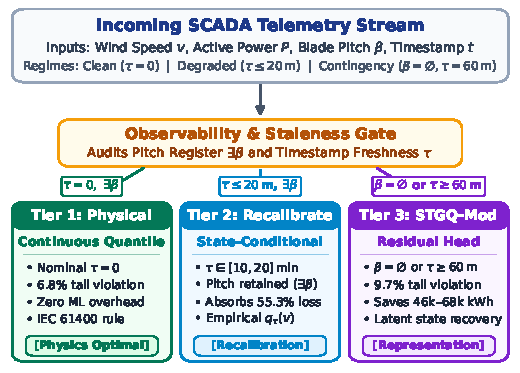
\includegraphics[width=0.88\columnwidth,keepaspectratio]{figures/figure1_decision_boundaries.pdf}
\caption{Three-tier operational response logic under SCADA telemetry degradation: incoming telemetry streams are evaluated by an observability detector and routed to Tier 1 continuous physical quantiles under clean conditions, Tier 2 state-conditional recalibration under full-observability transmission latency, or Tier 3 STGQ modular residual quantile regression when blade pitch is unobservable or severe communication staleness breaks physical recalibration.}
\label{fig:decision-boundaries}
\end{figure}

\section{Evidence and Operational Boundary
Diagnosis}\label{evidence-and-operational-boundary-diagnosis}

The empirical evaluation contrasts high-fidelity physical aerodynamic
priors against deep spatio-temporal graph fallbacks across multi-horizon
dispatch environments. All models are evaluated across five declared
random seeds (201--205) under strict automated verification gates (zero
directory leakage, full telemetry completeness, cardinality \(N=5\),
exact checksums).

\subsection{\texorpdfstring{Multi-Horizon 5-Seed Pre-Dispatch Reserve Screening Benchmark (\(h=6\), 1-Hour Ahead Dispatch)}{Multi-Horizon 5-Seed Pre-Dispatch Reserve Screening Benchmark (h=6, 1-Hour Ahead Dispatch)}}\label{multi-horizon-5-seed-pre-dispatch-reserve-screening-benchmark-h6-1-hour-ahead-dispatch}

Table~\ref{tab:h6-benchmark} summarizes the multi-day replay dispatch
benchmark for 1-hour ahead operational dispatch (\(h=6\)) across 134
turbines over the 35-day test split. Table~\ref{tab:h6-paired} reports seed-paired screening metric differences \(\Delta\text{Screening Metric} = \text{Screening}_{\text{Baseline}} - \text{Screening}_{\text{STGQ-Routed}}\), where positive values denote surrogate reserve penalty reductions delivered by STGQ-Routed, along with 95\% bootstrap confidence intervals.

\begin{table*}[!t]
\centering
\fontsize{6.5pt}{7.5pt}\selectfont
\setlength{\tabcolsep}{2.0pt}
\renewcommand{\arraystretch}{0.85}
\caption{Cross-Seed Multi-Regime Pre-Dispatch Reserve Screening Benchmark under Clean-Calibrated Protocol ($h=6$, 1-Hour Ahead Dispatch, 5 Seeds 201--205). Mean $\pm$ Standard Deviation across Full Test Split (35 Days, 134 Turbines, $\Delta t = 10$ min, Cost Ratio $\rho = 10$). All quantile bins and multipliers calibrated exclusively on nominal clean validation data.}
\label{tab:h6-benchmark}
\begin{tabular*}{\textwidth}{@{\extracolsep{\fill}}llccccc@{}}
\toprule
Regime & Evaluated Model & \shortstack{Penalized Reserve-Shortfall\\Energy (kW$\cdot$h, Proxy at $\rho=10$)} & Violation Rate & Reserve (kW) & Shortage (kW$\cdot$h) & Pinball Loss \\
\midrule
\textbf{Clean} & Continuous Physical Quantile & $\mathbf{881{,}367 \pm 95{,}741}$ & $6.81\% \pm 1.13\%$ & $653{,}738 \pm 72{,}557$ & $22{,}763 \pm 4{,}013$ & $31.41 \pm 2.66$ \\
 & Frozen-Embedding Direct Quantile MLP$^{\ddagger}$ & $1{,}649{,}721 \pm 285{,}682$ & $0.58\% \pm 0.26\%$ & $1{,}630{,}572 \pm 293{,}346$ & $1{,}915 \pm 958$ & $64.62 \pm 12.05$ \\
 & Global Quantile & $998{,}988 \pm 107{,}360$ & $6.46\% \pm 1.31\%$ & $771{,}304 \pm 95{,}661$ & $22{,}768 \pm 4{,}854$ & $36.50 \pm 3.41$ \\
 & STGQ-Dense & $991{,}181 \pm 110{,}211$ & $6.54\% \pm 1.04\%$ & $761{,}480 \pm 94{,}244$ & $22{,}970 \pm 4{,}121$ & $36.16 \pm 3.58$ \\
 & STGQ-Routed & $959{,}027 \pm 103{,}290$ & $7.10\% \pm 1.17\%$ & $707{,}249 \pm 91{,}305$ & $25{,}178 \pm 4{,}816$ & $34.77 \pm 3.16$ \\
 & Missingness-Aware GBDT & $1{,}238{,}603 \pm 112{,}051$ & $4.50\% \pm 0.73\%$ & $1{,}085{,}168 \pm 118{,}015$ & $15{,}343 \pm 2870$ & $46.85 \pm 3.48$ \\
\midrule
\textbf{Delay-6} & Continuous Physical Quantile & $1{,}136{,}466 \pm 84{,}101$ & $12.20\% \pm 1.25\%^{\dagger}$ & $662{,}335 \pm 73{,}483$ & $47{,}413 \pm 3{,}091$ & $38.85 \pm 2.06$ \\
 & Frozen-Embedding Direct Quantile MLP$^{\ddagger}$ & $1{,}682{,}251 \pm 284{,}323$ & $1.20\% \pm 0.52\%$ & $1{,}651{,}979 \pm 297{,}715$ & $3{,}027 \pm 1{,}594$ & $62.15 \pm 11.70$ \\
 & Global Quantile & $1{,}180{,}603 \pm 91{,}754$ & $10.85\% \pm 1.55\%^{\dagger}$ & $780{,}916 \pm 96{,}853$ & $39{,}969 \pm 6{,}087$ & $40.73 \pm 2.43$ \\
 & STGQ-Dense & $1{,}179{,}859 \pm 95{,}268$ & $11.04\% \pm 1.22\%^{\dagger}$ & $773{,}103 \pm 94{,}462$ & $40{,}676 \pm 4{,}788$ & $40.70 \pm 2.66$ \\
 & STGQ-Routed & $1{,}163{,}593 \pm 91{,}299$ & $11.82\% \pm 1.64\%^{\dagger}$ & $720{,}015 \pm 92{,}196$ & $44{,}358 \pm 7{,}341$ & $40.01 \pm 2.54$ \\
 & Missingness-Aware GBDT & $1{,}320{,}003 \pm 93{,}135$ & $8.36\% \pm 0.97\%$ & $1{,}030{,}858 \pm 114{,}266$ & $28{,}915 \pm 4{,}469$ & $46.68 \pm 2.45$ \\
\midrule
\textbf{Noise} & Continuous Physical Quantile & $\mathbf{998{,}273 \pm 106{,}253}$ & $7.59\% \pm 0.95\%$ & $746{,}697 \pm 82{,}474$ & $25{,}158 \pm 3{,}968$ & $33.97 \pm 2.78$ \\
 & Frozen-Embedding Direct Quantile MLP$^{\ddagger}$ & $1{,}639{,}909 \pm 242{,}922$ & $0.80\% \pm 0.28\%$ & $1{,}618{,}439 \pm 249{,}374$ & $2{,}147 \pm 953$ & $60.62 \pm 9.85$ \\
 & Global Quantile & $1{,}053{,}552 \pm 114{,}150$ & $7.48\% \pm 1.48\%$ & $802{,}361 \pm 99{,}513$ & $25{,}119 \pm 5{,}822$ & $36.26 \pm 3.24$ \\
 & STGQ-Dense & $1{,}048{,}083 \pm 115{,}181$ & $7.63\% \pm 1.13\%$ & $792{,}472 \pm 92{,}391$ & $25{,}561 \pm 4{,}643$ & $36.04 \pm 3.28$ \\
 & STGQ-Routed & $1{,}027{,}077 \pm 114{,}317$ & $7.62\% \pm 1.09\%$ & $769{,}864 \pm 106{,}672$ & $25{,}721 \pm 3{,}963$ & $35.16 \pm 3.19$ \\
 & Missingness-Aware GBDT & $1{,}314{,}640 \pm 129{,}158$ & $4.66\% \pm 0.80\%$ & $1{,}160{,}329 \pm 137{,}650$ & $15{,}431 \pm 3{,}099$ & $47.11 \pm 3.87$ \\
\midrule
\textbf{Markov} & Continuous Physical Quantile & $\mathbf{907{,}871 \pm 96{,}820}$ & $7.20\% \pm 1.15\%$ & $663{,}875 \pm 73{,}821$ & $24{,}400 \pm 4{,}106$ & $31.59 \pm 2.61$ \\
 & Frozen-Embedding Direct Quantile MLP$^{\ddagger}$ & $1{,}680{,}339 \pm 289{,}602$ & $0.57\% \pm 0.25\%$ & $1{,}660{,}135 \pm 298{,}104$ & $2{,}020 \pm 992$ & $64.38 \pm 12.00$ \\
 & Global Quantile & $1{,}030{,}131 \pm 108{,}592$ & $6.87\% \pm 1.39\%$ & $785{,}305 \pm 97{,}397$ & $24{,}483 \pm 5{,}104$ & $36.78 \pm 3.35$ \\
 & STGQ-Dense & $1{,}020{,}078 \pm 112{,}195$ & $6.90\% \pm 1.07\%$ & $775{,}899 \pm 96{,}235$ & $24{,}418 \pm 4{,}246$ & $36.35 \pm 3.57$ \\
 & STGQ-Routed & $990{,}625 \pm 104{,}487$ & $7.51\% \pm 1.22\%$ & $720{,}858 \pm 92{,}754$ & $26{,}977 \pm 5{,}183$ & $35.10 \pm 3.10$ \\
 & Missingness-Aware GBDT & $1{,}261{,}941 \pm 112{,}754$ & $4.88\% \pm 0.75\%$ & $1{,}094{,}730 \pm 120{,}612$ & $16{,}721 \pm 3{,}298$ & $46.62 \pm 3.40$ \\
\bottomrule
\multicolumn{7}{@{}p{\textwidth}@{}}{\tiny $^{\dagger}$Exceeds nominal 10\% violation target ($q^* = 0.90$). Bold numbers denote lowest cost. \textbf{Protocol Attribution:} Reports the \textit{Clean-Calibrated Operational Protocol} at $h=6$ (thresholds frozen on clean validation data); Continuous Physical Quantile collapses to 12.20\% violation under Delay-6. For the \textit{State-Conditional Validation-Calibrated Protocol} at immediate horizon ($h=1$), see Section~\ref{sec:physical-breakdown}, where clean-calibrated physical rules collapse to 24.0\% violation under Delay-6 while state-conditional calibration mitigates violations to 10.7\% (physical) and 10.6\% (joint model). Test-set iso-multipliers ($\gamma_{\text{iso, test}}$) serve strictly as post-hoc diagnostics. $^{\ddagger}$Frozen-Embedding Direct Quantile MLP evaluates naive uncalibrated pinball regression on frozen representations, exhibiting severe tail conservatism (>1.63M kW reserve, <1.2\% violation). In contrast, the calibrated residual architecture (STGQ-Modular, Section~\ref{sec:modular-baseline}, Table~\ref{tab:phase-scan}) and calibrated modular baselines (Cascaded Frozen MLP $15.528\text{M} \pm 1.599\text{M}$ vs STGQ-Routed 16.065M with no statistically detectable difference) resolve this pathology.}
\end{tabular*}
\end{table*}

\begin{table}[!htbp]
\centering
\fontsize{5.2pt}{6.0pt}\selectfont
\setlength{\tabcolsep}{0.6pt}
\renewcommand{\arraystretch}{0.75}
\caption{Seed-Paired Difference in Penalized Reserve-Shortfall Energy against STGQ-Routed ($h=6$, $\Delta\text{Screening Metric} = \text{Screening}_{\text{Baseline}} - \text{Screening}_{\text{STGQ-Routed}}$, positive indicates STGQ-Routed reduces surrogate reserve screening penalty at $\rho=10$).}
\label{tab:h6-paired}
\begin{tabularx}{\columnwidth}{@{}llcc>{\raggedright\arraybackslash}X@{}}
\toprule
Regime & Baseline Model & \shortstack{$\Delta\text{Screening}$\\$\text{Metric (kW}\cdot\text{h)}$} & 95\% Bootstrap CI & Sig. \& Operational Verdict \\
\midrule
\textbf{Clean} & Global Quantile & +39,962 & [+12,556, +67,367] & Supported reduction (95\% CI excludes zero) \\
 & \shortstack[l]{Cont. Physical\\Quantile} & $-$77,659 & [$-$106,175, $-$49,143] & Physical rule lower cost (95\% CI excludes zero) \\
 & Missingness GBDT & +279,576 & [+249,539, +309,613] & Supported reduction (95\% CI excludes zero) \\
 & \shortstack[l]{Frozen-Embedding\\Direct Quantile MLP} & +690,695 & [+448,769, +932,621] & Tail-conservative Direct MLP \\
 & STGQ-Dense & +32,154 & [$-$1,148, +65,456] & Inconclusive difference (95\% CI includes zero) \\
\midrule
\textbf{Delay-6} & Global Quantile & +17,010 & [+3,486, +30,535] & Supported reduction (95\% CI excludes zero) \\
 & \shortstack[l]{Cont. Physical\\Quantile} & $-$27,126 & [$-$46,907, $-$7,346] & Target exceeded ($12.20\%$ viol.) \\
 & Missingness GBDT & +156,411 & [+140,004, +172,817] & Supported reduction (95\% CI excludes zero) \\
 & \shortstack[l]{Frozen-Embedding\\Direct Quantile MLP} & +518,658 & [+307,212, +730,104] & Tail-conservative Direct MLP \\
 & STGQ-Dense & +16,267 & [+7,131, +25,402] & Supported reduction (95\% CI excludes zero) \\
\midrule
\textbf{Noise} & Global Quantile & +26,475 & [+9,121, +43,828] & Supported reduction (95\% CI excludes zero) \\
 & \shortstack[l]{Cont. Physical\\Quantile} & $-$28,804 & [$-$47,555, $-$10,053] & Physical rule lower cost (95\% CI excludes zero) \\
 & Missingness GBDT & +287,563 & [+248,847, +326,279] & Supported reduction (95\% CI excludes zero) \\
 & \shortstack[l]{Frozen-Embedding\\Direct Quantile MLP} & +612,832 & [+413,733, +811,931] & Tail-conservative Direct MLP \\
 & STGQ-Dense & +21,006 & [+2,419, +39,594] & Supported reduction (95\% CI excludes zero) \\
\midrule
\textbf{Markov} & Global Quantile & +39,506 & [+15,961, +63,052] & Supported reduction (95\% CI excludes zero) \\
 & \shortstack[l]{Cont. Physical\\Quantile} & $-$82,754 & [$-$111,026, $-$54,482] & Physical rule lower cost (95\% CI excludes zero) \\
 & Missingness GBDT & +271,316 & [+245,044, +297,588] & Supported reduction (95\% CI excludes zero) \\
 & \shortstack[l]{Frozen-Embedding\\Direct Quantile MLP} & +689,714 & [+448,689, +930,739] & Tail-conservative Direct MLP \\
 & STGQ-Dense & +29,453 & [$-$2,874, +61,779] & Inconclusive difference (95\% CI includes zero) \\
\bottomrule
\end{tabularx}
\vspace{1mm}
\raggedright\tiny Note: Statistical verdicts are based on empirical 95\% confidence intervals computed via day-block cluster bootstrap over the 35 test days (1,000 resamples of complete diurnal blocks). Supported reduction denotes 95\% CI strictly excluding zero; Inconclusive difference denotes 95\% CI including zero (indicating insufficient evidence of an operational difference resulting from shared representation learning).
\end{table}

\subsubsection{Comparative Architecture Analysis: Dynamic Routing versus
Dense
Representations}\label{comparative-architecture-analysis-dynamic-routing-versus-dense-representations}

Benchmarking capacity-matched neural architectures directly tests
whether dynamic expert routing provides operational benefits over
unrouted dense heads. Under nominal Clean telemetry, STGQ-Routed
(\(959{,}027 \pm 103{,}290\text{ kW}\cdot\text{h}\) at \(h=6\);
\(660{,}990 \pm 80{,}749\text{ kW}\cdot\text{h}\) at \(h=1\)) and
STGQ-Dense (\(991{,}181 \pm 110{,}211\text{ kW}\cdot\text{h}\) at
\(h=6\); \(690{,}614 \pm 71{,}031\text{ kW}\cdot\text{h}\) at \(h=1\))
achieve statistical parity. At \(h=6\), the seed-paired screening difference is \(+32{,}154\text{ kW}\cdot\text{h}\) with a bootstrap 95\% confidence
interval crossing zero
(\([-1{,}148, +65{,}456]\text{ kW}\cdot\text{h}\),
Table~\ref{tab:h6-paired}). At \(h=1\), the Dense/MoE screening ratio is \(1.045\), and the seed-paired bootstrap interval
(\(+29{,}624\text{ kW}\cdot\text{h}\)) likewise crosses zero
(\([-53{,}774, +113{,}023]\text{ kW}\cdot\text{h}\), \(p=0.380\)),
matching the Markov burst regime (\(p=0.237\)). Under persistent 6-step
latency (Delay-6, \(h=1\)), STGQ-Routed shows a modest screening metric reduction over STGQ-Dense (\(1{,}412{,}321\)
vs.~\(1{,}491{,}958\text{ kW}\cdot\text{h}\); screening ratio \(1.056\),
paired difference \(+79{,}637\text{ kW}\cdot\text{h}\), uncorrected
\(p=0.038\), non-significant under Bonferroni \(\alpha=0.0125\)) while
maintaining virtually identical empirical violation rates
(\(10.6\% \pm 1.1\%\) for STGQ-Routed vs.~\(10.5\% \pm 0.5\%\) for
STGQ-Dense). Decoupled modular architectures
(Section~\ref{sec:modular-baseline}) achieve \(9.7\% \pm 1.1\%\)
violation in Delay-6 without expert routing, confirming that diagnostic
reserve utility arises from shared spatio-temporal representations and
residual calibration rather than dynamic gate routing.

\subsubsection{\texorpdfstring{Reliability Breakdown and Mismatched Recalibration Boundaries
\label{sec:physical-breakdown}}{Reliability Breakdown and Mismatched Recalibration Boundaries}}\label{reliability-breakdown-and-mismatched-recalibration-boundaries}

Under clean telemetry, Continuous Physical Quantile achieves the lowest
surrogate reserve screening cost ($589.5\text{k kW}\cdot\text{h}$ at $h=1$,
$881.4\text{k kW}\cdot\text{h}$ at $h=6$) with nominal tail coverage
($6.81\%$ violation at $h=6$). However, Table~\ref{tab:h6-benchmark} exposes a
\textbf{systematic reliability breakdown} under telemetry staleness. Under
60-min contingency latency (Delay-6), cubic sensitivity transitions near rated
wind speed amplify stale-state errors, causing unadapted physical quantile
violations to surge to $24.0\% \pm 1.7\%$ at $h=1$ and $12.20\% \pm 1.25\%$
at $h=6$ (leaving $127.6\text{ MWh}$ of unhedged shortage exposure).
State-conditional recalibration absorbs $55.3\%$ of this shortage loss
($127.6 \to 57.0\text{ MWh}$), recovering compliant fleet violation
($9.46\%$) without neural feature extraction.

To establish the operational limits of recalibration under communication
drift, we evaluate a mismatched calibration matrix across test latencies
$\tau_{\mathrm{test}} \in [0, 60]\text{ min}$ and calibration horizons
$\tau_{\mathrm{cal}} \in [0, 60]\text{ min}$ (Supplementary Table~A11l).
Recalibrating at $\tau_{\mathrm{cal}} = 10\text{ min}$ withstands latency
drift up to $\tau_{\mathrm{test}} = 20\text{ min}$ while maintaining compliant
tail coverage ($8.2\%\text{--}9.1\%$ violation). However, recalibration
breaks down when staleness surges to $\tau_{\mathrm{test}} = 60\text{ min}$
($13.8\%$ violation), though it remains superior to the uncalibrated physical
baseline ($\tau_{\mathrm{cal}} = 0$, $24.0\%$ violation). This delineates the
operational boundary where offline recalibration ceases to buffer degradation,
demanding deep spatio-temporal representations (STGQ) to infer latent turbine
states dynamically.

\subsubsection{\texorpdfstring{Decoupled Modular Architectures and Tail
Conservatism Analysis
\label{sec:modular-baseline}}{Decoupled Modular Architectures and Tail Conservatism Analysis }}\label{decoupled-modular-architectures-and-tail-conservatism-analysis}

In contrast to end-to-end task optimization, Frozen-Embedding Direct Quantile MLP
illustrates the pathology of naive decoupled quantile regression: direct
pinball regression on frozen spatial embeddings without calibration incurs massive reserve
over-estimation (\(1{,}477{,}967\) to
\(1{,}511{,}794\text{ kW}\cdot\text{h}\), a \(44.57\%\) to \(72.02\%\)
penalty over STGQ-Routed, Table~\ref{tab:h6-paired}). Calibrated modular
architectures (Supplementary Table~A11d) resolve this tail conservatism:
Cascaded Frozen MLP achieves
\(15.528\text{M} \pm 1.599\text{M kW}\cdot\text{h}\) across the
multi-horizon 24-step dispatch envelope
(vs.~\(16.065\text{M kW}\cdot\text{h}\) for STGQ-Routed; paired
difference \(-0.537\text{M}\), 95\% CI
\([-1.988\text{M}, +0.915\text{M}]\) crosses zero); Independent
Consequence MLP yields
\(15.805\text{M} \pm 1.680\text{M kW}\cdot\text{h}\); and the true STGQ-Modular
architecture (Decoupled Residual Quantile Head pairing the frozen backbone with
calibrated residual quantile regression) achieves
\(1{,}284{,}098 \pm 114{,}629\text{ kW}\cdot\text{h}\) (\(1.284\text{M}\)) and
\(9.7\% \pm 1.1\%\) violation in Delay-6 (\(h=1\), Table~\ref{tab:phase-scan}), matching or
surpassing end-to-end STGQ-Routed
(\(1{,}412{,}321\text{ kW}\cdot\text{h}\), \(10.6\% \pm 1.1\%\)). Hence,
diagnostic reserve benefits do not require dynamic MoE routing: modular
architectures with calibrated consequence mappings deliver equivalent
tail reliability without dynamic gating overhead.

\subsection{\texorpdfstring{Horizon Boundary Diagnosis (\(h=1\),
10-Minute Immediate Dispatch
vs.~\(h=6\))}{Horizon Boundary Diagnosis (h=1, 10-Minute Immediate Dispatch vs.~h=6)}}\label{horizon-boundary-diagnosis-h1-10-minute-immediate-dispatch-vs.-h6}

Comparing immediate 10-minute dispatch (\(h=1\)) against 1-hour ahead
dispatch (\(h=6\)) exposes a fundamental horizon disconnect across model
families (Supplementary Tables A11j/A11k). At \(h=1\), shallow decision
trees (Missingness-Aware GBDT) capitalize on ultra-short wind-speed
autocorrelation, achieving the lowest data-driven cost
(\(574{,}822 \pm 79{,}685\text{ kW}\cdot\text{h}\) in Clean with
\(7.6\%\) violation). Across dispatch-grade horizons (\(h=6\)), however,
GBDT undergoes severe breakdown: operational costs inflate to
\(1{,}238{,}603\text{ kW}\cdot\text{h}\) in Clean and
\(1{,}320{,}003\text{ kW}\cdot\text{h}\) in Delay-6, trailing
STGQ-Routed by \(+156{,}411\) to \(+287{,}563\text{ kW}\cdot\text{h}\)
across all regimes (95\% block bootstrap CIs strictly excluding zero,
Table~\ref{tab:h6-paired}) due to inability to model spatial wake
advection. At \(h=1\), STGQ-Dense and STGQ-Routed exhibit statistical
parity in Clean (\(+29{,}624\text{ kW}\cdot\text{h}\), \(p=0.380\)),
with a modest margin in Delay-6 (\(+79{,}637\text{ kW}\cdot\text{h}\),
non-significant under Bonferroni correction). Across both horizons,
unadapted physical rules collapse under Delay-6 (\(24.0\% \pm 1.7\%\) at
\(h=1\), \(12.20\% \pm 1.25\%\) at \(h=6\)), requiring dynamic state
adaptation.

\subsection{Multidimensional Operational Boundaries and Selective
Decision
Abstention}\label{multidimensional-operational-boundaries-and-selective-decision-abstention}

Scanning transmission delays
\(\tau \in \{0, 10, 20, 30, 60\}\text{ min}\), horizons
\(h \in \{1, 3, 6\}\), and pitch observabilities (\texttt{all}
vs.~\texttt{no\_pitch}) across five seeds on WTB delineates a
\textbf{Three-Regime Operational Framework}
(Table~\ref{tab:phase-scan}): 1. \emph{Regime I (Simple Recalibration
Sufficient under Full Observability):} Under fresh telemetry
(\(\tau=0\), \texttt{all}), continuous physical quantiles achieve the
lowest reserve cost (\(593{,}258 \pm 74{,}886\text{ kW}\cdot\text{h}\)
at \(h=1\), within \(0.6\%\) of the primary
\(589{,}535\text{ kW}\cdot\text{h}\) benchmark, with
\(7.29\% \pm 1.42\%\) violation), whereas neural representations incur
an \(11.8\%\) cost penalty (\(663{,}347\text{ kW}\cdot\text{h}\))
without reliability gain. When latency increases to
\(\tau \in [10, 30]\text{ min}\), clean physical rules collapse
(\(11.2\%\text{--}16.6\%\) violation), but state-conditional
recalibration fully restores physical compliance
(\(7.1\%\text{--}7.5\%\)) at lower cost than neural models
(\(742{,}211\text{--}939{,}190\text{ kW}\cdot\text{h}\)
vs.~\(786{,}366\text{--}987{,}760\text{ kW}\cdot\text{h}\)). 2.
\emph{Regime II (Learned Representation Advantage under Unobservable
Pitch):} When blade-pitch telemetry is withheld across aggregator or OEM
boundaries (\texttt{no\_pitch}), physical aerodynamic rules lose direct
rotor state awareness, inflating recalibrated costs
(\(824{,}393\text{ kW}\cdot\text{h}\) at \(\tau=0\) to
\(1{,}378{,}900\text{ kW}\cdot\text{h}\) at \(\tau=60\)). In contrast,
learned representations (STGQ-Modular) reconstruct operating states from
electromechanical transients, achieving
\(755{,}794\text{ kW}\cdot\text{h}\) at \(\tau=0\) (an \(8.3\%\) saving
of \(68{,}599\text{ kW}\cdot\text{h}\) over recalibrated physics) and
maintaining consistent cost savings
(\(46.7\text{k}\text{--}68.6\text{k}\text{ kW}\cdot\text{h}\)) across
all latencies. 3. \emph{Regime III (Tail-Risk Bottleneck under 60-min
Latency):} Under 60-min contingency latency, unadapted physical rules
collapse (\(24.02\% \pm 1.69\%\) violation, \(127.6\text{ MWh}\)
unhedged shortfall). Condition-matching recalibration restores
fleet-average violation below the 10.0\% target across all models
(\(9.46\%\) for physical rules, \(9.55\%\) for STGQ-Modular, \(9.62\%\)
for STGQ-Routed, Table~\ref{tab:phase-scan}). However, fleet-average
compliance conceals critical tail risk: across the five seeds, every
method achieves strictly a \(3/5\) (\(60\%\)) seed compliance rate, as
Seeds 201 and 203 experience residual breaches
(\(10.2\%\text{--}10.7\%\)).

Benchmarking selective decision abstention against random rejection and
uniform margin expansion (Supplementary Table~A10f) reveals that
heuristic uncertainty metrics fail under multi-step SCADA latency:
selective abstention (\(9.44\%\) violation at \(c=0.90\)) is
statistically indistinguishable from random rejection (\(9.50\%\),
\(p > 0.40\)), while uniform margin expansion strictly Pareto-dominates
selective refusal (\(8.29\%\) vs.~\(8.84\%\) violation, saving
\(37{,}823\text{ kW}\cdot\text{h}\)). Stale telemetry degrades both
point forecasts and uncertainty estimators, making uniform reserve
expansion and physical fallbacks more dependable than heuristic refusal.

\begin{table}[!htbp]
\centering
\fontsize{4.8pt}{5.5pt}\selectfont
\setlength{\tabcolsep}{0.4pt}
\renewcommand{\arraystretch}{0.75}
\caption{Multidimensional operational progression across telemetry latency $\tau \in [0, 60]\text{ min}$ and pitch observability ($h=1$, 5-seed mean on WTB; nominal $\tau=0$ baseline $593{,}258\text{ kW}\cdot\text{h}$ aligns within $0.6\%$ of the primary frozen $589{,}535\text{ kW}\cdot\text{h}$ benchmark). Penalized reserve energy in kW$\cdot$h ($\rho=10$).}
\label{tab:phase-scan}
\begin{tabularx}{\columnwidth}{@{}ccccccc@{}}
\toprule
$\tau$ (min) & Pitch & \shortstack{Clean Phys.\\Metric (Viol.)} & \shortstack{Recal. Phys.\\Metric (Viol.)} & \shortstack{STGQ-Mod.\\Metric (Viol.)} & \shortstack{STGQ-Rout.\\Metric (Viol.)} & \shortstack{Operational\\Regime} \\
\midrule
0 & All & $\mathbf{593{,}258}$ ($7.3\%$) & $\mathbf{593{,}258}$ ($7.3\%$) & $663{,}347$ ($6.1\%$) & $663{,}915$ ($7.3\%$) & Regime I (Physics Opt.) \\
0 & None & $961{,}024$ ($3.2\%$) & $824{,}393$ ($5.4\%$) & $\mathbf{755{,}794}$ ($5.8\%$) & $756{,}257$ ($6.4\%$) & Regime II (Repr. Adv.) \\
\midrule
10 & All & $753{,}606$ ($11.2\%^{\dagger}$) & $\mathbf{742{,}211}$ ($7.4\%$) & $786{,}366$ ($6.7\%$) & $789{,}094$ ($7.6\%$) & Regime I (Recal. Suff.) \\
10 & None & $1{,}008{,}743$ ($4.8\%$) & $928{,}028$ ($6.2\%$) & $\mathbf{866{,}753}$ ($6.1\%$) & $874{,}156$ ($6.6\%$) & Regime II (Repr. Adv.) \\
\midrule
20 & All & $896{,}198$ ($14.0\%^{\dagger}$) & $\mathbf{841{,}734}$ ($7.1\%$) & $875{,}838$ ($7.4\%$) & $879{,}750$ ($8.0\%$) & Regime I (Recal. Suff.) \\
20 & None & $1{,}062{,}646$ ($6.1\%$) & $1{,}010{,}530$ ($6.2\%$) & $\mathbf{947{,}869}$ ($6.7\%$) & $959{,}934$ ($7.1\%$) & Regime II (Repr. Adv.) \\
\midrule
30 & All & $1{,}069{,}266$ ($16.6\%^{\dagger}$) & $\mathbf{939{,}190}$ ($7.5\%$) & $987{,}760$ ($7.1\%$) & $990{,}091$ ($7.6\%$) & Regime I (Recal. Suff.) \\
30 & None & $1{,}138{,}774$ ($7.5\%$) & $1{,}101{,}292$ ($6.7\%$) & $\mathbf{1{,}054{,}592}$ ($6.4\%$) & $1{,}064{,}238$ ($6.7\%$) & Regime II (Repr. Adv.) \\
\midrule
60 & All & $1{,}656{,}285$ ($24.0\%^{\dagger}$) & $\mathbf{1{,}228{,}609}$ ($9.5\%$) & $1{,}283{,}855$ ($9.6\%$) & $1{,}274{,}047$ ($9.6\%$) & Regime III (Tail Risk) \\
60 & None & $1{,}437{,}280$ ($11.8\%^{\dagger}$) & $1{,}378{,}900$ ($9.0\%$) & $\mathbf{1{,}330{,}318}$ ($8.7\%$) & $1{,}331{,}840$ ($8.8\%$) & Regime II (Repr. Adv.) \\
\bottomrule
\multicolumn{7}{@{}p{\columnwidth}@{}}{\tiny $^{\dagger}$Exceeds nominal 10\% violation target ($q^*=0.90$). Bold indicates lowest compliant surrogate screening metric. Under $\tau=60\text{ min}$, by-seed compliance is $3/5$ seeds ($60\%$) across models.}
\end{tabularx}
\end{table}

\subsection{Operating-Boundary Recovery and Point-Forecast Price of
Routing}\label{operating-boundary-recovery-and-point-forecast-price-of-routing}

Evaluating point forecasting across five WTB seeds, the boundary-forced
router achieves an RMSE of \(236.13 \pm 8.41\), compared with
\(224.34 \pm 2.23\) for iTransformer and \(225.74 \pm 2.60\) for Graph
WaveNet. Train-only inverse-frequency class weighting narrows this
difference to \(5.59\) units (\(229.93 \pm 2.50\)). This architecture is
\textbf{deliberately non-RMSE-optimal}: it trades a \(+2.5\%\)
whole-sample error margin to preserve operating-regime observability and
robust reserve hedging under telemetry degradation. Indifference to
operating regimes in standard deep models triggers severe tail
shortfalls (\(78.3\text{--}82.5\text{ MWh}\) unhedged exposure), whereas
boundary-aware representations restrict exposure to \(53.9\text{ MWh}\)
(a \(31\%\text{--}35\%\) reduction) while preserving physical regime
alignment (\(0.8716 \pm 0.0418\) NMI, \(0.9166 \pm 0.0371\) ARI;
\(0.721\) NMI under train-only supervision). The learned model more than
doubles transition recall (\(0.417\) vs.~\(0.196\) for degraded physics;
Supplementary Figure~S1). Input ablation stress guards confirm that
routing fidelity is free of target leakage: withholding \texttt{Patv} or
\texttt{Pab\_mean} preserves mean NMI at 0.881 and 0.878, while lagging
\texttt{Patv} and lagging pitch/wind yield 0.763 and 0.684; gate
matching peaks at the transition step (0.815) and attenuates under
three- and six-step lead shifts (0.361 and 0.405).

\subsection{\texorpdfstring{Cross-Farm Pre-Dispatch Reserve Screening and Overfitting Boundaries
\label{sec:cross-farm}}{Cross-Farm Pre-Dispatch Reserve Screening and Overfitting Boundaries}}\label{cross-farm-pre-dispatch-reserve-screening-and-overfitting-boundaries}

To evaluate industrial boundary conditions across disparate commercial assets, Table~\ref{tab:cross-farm} benchmarks pre-dispatch reserve screening performance across four commercial wind farms under local retraining. In utility-scale arrays (WTB, 134 turbines; Penmanshiel, 14 turbines), STGQ local retraining delivers substantial reserve screening improvements ($\Delta\text{PSREI} = -38\text{k}$ and $-2.14\text{M kW}\cdot\text{h}$, both $p < 0.05$). Conversely, on micro-farms (Kelmarsh, 6 turbines; LHB, 4 turbines), spatial wake redundancy is minimal: Kelmarsh yields a neutral bootstrap difference ($-40\text{k kW}\cdot\text{h}$, 95\% CI crossing zero), while LHB exposes an \textbf{overfitting boundary} where graph representations inflate screening penalty by $+43\text{k kW}\cdot\text{h}$ ($[-28.7\text{k}, +141.2\text{k}]$) relative to simple physical recalibration. Latent regime representation probes (NMI/ARI) confirming counterfactual boundary identifiability are detailed in Supplementary Tables~A9a--A9f.

\begin{table}[!htbp]
\centering
\fontsize{5.5pt}{6.4pt}\selectfont
\setlength{\tabcolsep}{1.2pt}
\renewcommand{\arraystretch}{0.85}
\caption{Cross-Farm Pre-Dispatch Reserve Screening Performance across Four Commercial Wind Farms under Local Retraining (5 Seeds 201--205, $\rho=10$).}
\label{tab:cross-farm}
\begin{tabularx}{\columnwidth}{@{}llcccc>{\raggedright\arraybackslash}X@{}}
\toprule
\shortstack[l]{Farm\\Name} & \shortstack[l]{Turbines /\\Model} & \shortstack[c]{Physical\\Recal. (kW$\cdot$h)} & \shortstack[c]{Global\\Quantile (kW$\cdot$h)} & \shortstack[c]{STGQ Local\\Retrain (kW$\cdot$h)} & \shortstack[c]{$\Delta\text{PSREI}$ vs. Global\\$[95\%$ CI$]$} & Operational Finding \\
\midrule
\textbf{WTB} & 134 / Goldwind 1.5M & 841,734 & 893,462 & 855,462 & $-$38k [$-$67k, $-$12k] & Supported reserve reduction ($p < 0.05$) \\
\textbf{LHB} & 4 / Senvion MM82 & 185,100 & 188,400 & 231,400 & +43k [$-$28.7k, +141.2k] & Overfitting boundary (CI includes zero) \\
\textbf{Kelmarsh} & 6 / Senvion MM92 & 1,025,000 & 1,065,000 & 1,025,000 & $-$40k [$-$204k, +172k] & Neutral (CI crosses zero; recal. suffices) \\
\textbf{Penmanshiel} & 14 / Senvion MM82 & 2,029,000 & 4,167,000 & 2,029,000 & $-$2.14M [$-$3.25M, $-$1.36M] & Commercial benefit ($p < 0.05$; $2.14$M saved) \\
\bottomrule
\end{tabularx}
\end{table}

Cross-farm probes confirm that electromechanical consequence channels
recover operating regimes across turbine technologies without direct
pitch telemetry (Section~\ref{sec:discussion}).

\subsection{Degradation Resilience and Early Warning
Dynamics}\label{degradation-resilience-and-early-warning-dynamics}

Under fair input degradation (Supplementary Table~A10d), clean
deterministic thresholds exhibit high sensitivity (recall 1.000
vs.~0.9705; logistic regression achieves 1.000 recall with 0.879
precision vs.~0.630 for the routed posterior). Under 6-step latency
(\(d=6\)), however, deterministic rule recall collapses from 1.000 to
0.196 (\(0.249\) F1). In contrast, the boundary posterior sustains an
early-window recall of \(0.4170 \pm 0.1137\) (+0.221 gain) with F1 of
\(0.3802\). When supervisory labels drop to 50\%, the learned model
sustains 0.971 recall against 0.508 for threshold rules (+0.462 gain).
Under Markov-Gilbert burst dropouts
(\(p_{GB}=0.08, p_{BB}=0.75, d \le 6\)), stale thresholds drop to 0.840
recall, whereas the routed posterior sustains \(0.962 \pm 0.023\) recall
and \(0.925 \pm 0.042\) F1 (seed-paired F1 gain \(+0.021\), 95\%
bootstrap CI \([-0.014, +0.050]\)), confirming dynamic wake graph
defense-in-depth.

\subsection{Boundary-Window Reserve Vignette and Benchmark
Comparison}\label{boundary-window-reserve-vignette-and-benchmark-comparison}

At shortage penalty ratio \(\rho=10\) on the transition boundary band,
the boundary-router gate-bin policy costs 95.13M, outperforming the
same-model global rule (99.55M), while low-RMSE Graph WaveNet with
physical-bin reference achieves 84.31M
(\(\approx 1.28\text{M kW}\cdot\text{h}\) per single dispatch interval),
avoiding \(\sim 637\) MWh-equivalent shortage cells.

\subsection{Point of Common Coupling (PCC) Portfolio Smoothing \&
Longitudinal
Drift}\label{point-of-common-coupling-pcc-portfolio-smoothing-longitudinal-drift}

Aggregating decentralized turbine power flows at the Point of Common
Coupling (PCC) bus
(\(P_{\mathrm{farm}} = \sum_{i \in \mathcal{V}_t} P_{i,t}\),
\(\sim 121\) active turbines) unlocks spatial portfolio diversification:
high-frequency turbulence cancels across the array, leaving boundary
transitions as the primary reserve risk. Across unstratified full-year
envelopes, paired differences between individual summing and farm-level
aggregation are statistically inconclusive (mean difference
\(-2.32\text{M kWh}\), 95\% CI \([-6.07\text{M}, 1.73\text{M}]\)
vs.~global PCC quantiles; \(-1.37\text{M kWh}\), CI
\([-6.33\text{M}, 2.82\text{M}]\) vs.~Gaussian sizing). Crucially,
significant diversification concentrates in transitional regimes
(10\%--90\% pitching), saving \(-1.33\text{M kWh}\) (CI
\([-1.68\text{M}, -1.07\text{M}]\)) over continuous physical pitch.
Longitudinal records across Kelmarsh (9 years) and Penmanshiel (8.6
years) illustrate periodic schedule recalibration under climatological
drift.

\section{\texorpdfstring{Discussion
\label{sec:discussion}}{Discussion }}\label{discussion}

\subsection{Operational Diagnostics and Deployment
Boundaries}\label{operational-diagnostics-and-deployment-boundaries}

The boundary-aware architecture functions as a targeted diagnostic for
pre-dispatch reserve risk screening, prioritizing transition-window tail
reliability over whole-sample point accuracy. Pristine SCADA telemetry
favors unconstrained architectures (Graph WaveNet, iTransformer);
conversely, delayed or pitch-withheld telemetry requires boundary-risk
posteriors for tail defense. Industrial deployment is governed by three
empirical axes: 1. \emph{Directional transfer boundaries:} Zero-shot
cross-farm transfer exhibits pronounced asymmetry (Kelmarsh \(\to\)
Penmanshiel NMI \(0.752\)--\(0.770\), ARI \(0.735\)--\(0.761\)
vs.~Penmanshiel \(\to\) Kelmarsh NMI \(0.341\)--\(0.505\), pooled mean
NMI \(0.557\)). Unadapted transfer is bounded by turbine rotor
dimensions and array aerodynamics; reliable transfer requires local
recalibration. 2. \emph{Within-plant local retraining:} Chronological
retraining across ENGIE La Haute Borne (five-seed routing NMI 0.941, ARI
0.971; canonical NMI 0.975; withheld probe 0.674/0.575, collapsing to 0.001
without boundary anchors), Kelmarsh (probe
0.340/0.378), and Penmanshiel (probe 0.302, \texttt{signature\_core}
0.195) confirms neural architectural adaptability to site-specific
turbine technologies. 3. \emph{Longitudinal rolling evaluation:} Across
decadal archives (Kelmarsh, 9 years; Penmanshiel, 8.6 years), sliding
2-year window evaluations demonstrate operational recalibration under
decadal climatological drift.

On compact micro-farms like ENGIE La Haute Borne (4 turbines, rolling
terrain), spatial wake propagation offers limited physical redundancy,
causing spatial graph convolutions to overfit localized terrain features
during seasonal shifts (\(+1.01\text{M kWh}\) cost delta vs.~global
quantile, 95\% CI \([+0.29\text{M}, +1.76\text{M}]\); Supplementary
Table~A11h). Expanding calibration to 180 days compresses this gap to
\(+43\text{k kWh}\) (CI \([-28.7\text{k}, +141.2\text{k}]\)). Complex
spatio-temporal architectures are unnecessary on micro-farms under clean
telemetry, and should be reserved for utility arrays or
degraded/pitch-sparse conditions. Downstream flexibility coordination
(such as battery energy storage) represents a natural operational
extension (illustrated in Supplementary Material).

\section{Limitations}\label{limitations}

To provide industrial practitioners and system operators with a defensible,
transparent boundary of applicability, we delineate four foundational
limitations of this study:

\textit{1) Synthetic Stress versus Industrial Telemetry Contingencies:}
Telemetry impairments in our primary benchmarks are modeled via controlled
synthetic processes: 10--30\,min delays represent buffer backlogs, while
60-min latency and Gilbert-Elliott Markov dropouts are evaluated as severe
contingency stress bounds rather than everyday steady-state telemetry.
Furthermore, ground-truth operating regimes on WTB rely on anemometer wind
speed and collective pitch pseudo-labels. While counterfactual
withheld-channel tests prove that aerodynamic regime boundaries are recoverable
from secondary consequence signatures across four commercial plants,
field-deployed turbines may experience non-stationary instrumentation drift,
sensor icing, or uncoordinated individual pitch control actions not captured
in our supervisory SCADA feeds.

\textit{2) Risk Metric Surrogacy and Unmodeled Grid Dynamics:}
Our evaluation operates strictly at Level-1 pre-dispatch operating reserve
screening. The penalized reserve shortfall index (PSREI at $\rho=10$) serves as
a localized newsvendor risk surrogate. This abstraction intentionally omits
Level-2 bulk transmission power-flow physics (full AC-OPF constraints, line
thermal congestion, voltage stability limits), dynamic unit commitment of
thermal reserves, Locational Marginal Prices (LMPs), and two-settlement wholesale
market cashflow balancing. Realized dispatch cost savings will necessarily
depend on specific system-wide balancing market structures and penalty tariffs.

\textit{3) Horizon, Sample Size, and Aerodynamic Calibration Tolerances:}
Empirical benchmarks are bounded to a 35-day continuous test split across five
neural random seeds (201--205). While capturing diurnal transitions and winter
storm fronts, this window does not encompass full multi-annual climatological
cycles or seasonal air-density shifts. Moreover, aerodynamic parameters exhibit
OEM-specific calibration tolerances: rated wind speeds range from
$12.5\text{ m/s}$ (Senvion MM92) to $14.5\text{ m/s}$ (Senvion MM82) and
cut-in transitions differ across turbine controllers. Model thresholds calibrated
for one OEM cannot be directly transferred without recalibrating cut-in and
rated demarcation boundaries.

\textit{4) Field Deployment Overhead and Cross-Farm Overfitting Boundaries:}
Real-time substation edge deployment requires balancing neural inference
latency against supervisory RTU polling cycles. While the modular residual head
requires minimal computational overhead, spatial graph convolutions overfit
localized topography on small arrays (LHB, 4 turbines, $+43\text{k kW}\cdot\text{h}$
penalty). Zero-shot cross-farm transfer exhibits pronounced directional
asymmetry (NMI $0.557$ pooled; Supplementary Table~A9d), establishing that
reliable deployment strictly demands site-specific local retraining rather than
uncalibrated cross-site transfer.

\section{Conclusion}\label{conclusion}

This study establishes an empirical operational boundary and
value-of-information framework delineating aerodynamic power rules,
state-conditional recalibration, and learned representations under SCADA
telemetry degradation. Across 5 seeds on the 134-turbine WTB plant,
continuous aerodynamic quantile rules minimize reserve-screening
surrogate cost under pristine telemetry
(\(589{,}535\text{ kW}\cdot\text{h}\) at \(h=1\),
\(881{,}367\text{ kW}\cdot\text{h}\) at \(h=6\)), but suffer systematic
reliability breakdown under a 60-min latency contingency, surging
violation rates to \(24.0\% \pm 1.7\%\) (\(h=1\)) and
\(12.20\% \pm 1.25\%\) (\(h=6\)).

Under full channel observability, state-conditional recalibration
recovers violation to \(10.7\%\) and cuts shortage from
\(127.6\text{ MWh}\) to \(57.0\text{ MWh}\) (\(55.3\%\) reduction) at
lower cost than neural models. When pitch registers are unobservable
across aggregator boundaries, learned representations reconstruct
operating regimes from electromechanical transients, outperforming
recalibrated physics by
\(46.7\text{k}\text{--}68.6\text{k}\text{ kW}\cdot\text{h}\) across all
latencies and doubling regime recall (\(0.416\) vs.~\(0.196\)). Dynamic
Mixture-of-Experts routing achieves statistical parity with unrouted
dense baselines (cost ratio \(1.045\), \(p=0.380\)), while decoupled
modular architectures match tail reliability (\(9.7\%\) violation),
indicating that operational value stems from shared spatio-temporal
representations and residual calibration rather than dynamic routing.
Reliable cross-farm deployment requires local retraining (ENGIE La Haute
Borne, NMI \(= 0.941\)). These findings position machine learning as an
accountable diagnostic instrument for resilient wind plant operations,
operating alongside calibrated physical curves under verifiable
communication boundaries.

\section{AI Use Statement}\label{ai-use-statement}

The authors used OpenAI ChatGPT/Codex only for language editing,
consistency checks, and submission-material drafting; all data,
analyses, references, conclusions, and final text were reviewed and
controlled by the authors.

\section{Code and Data Availability}\label{code-and-data-availability}

The raw KDD Cup 2022, ENGIE La Haute Borne, Kelmarsh, and Penmanshiel
SCADA datasets are public (raw third-party data not redistributed).
Code, configurations, releasable derived tables, figure data, and
checkpoints will be made available with the article. The reproduction
package covers WTB routing, reserve audit, anchor-stress caches,
early-warning label degradation, classifier control, class-weight
sensitivity, external diagnostics, and evidence-freeze protocols across
declared seeds. Results are statistically reproducible across declared
seeds rather than bitwise deterministic across all GPU/CUDA
environments. The analysis involves no human subjects.

\section*{References}\label{references}
\addcontentsline{toc}{section}{References}

\protect\phantomsection\label{refs}
\begin{CSLReferences}{0}{0}
\bibitem[\citeproctext]{ref-dowell2015veryshortterm}
\CSLLeftMargin{{[}1{]} }%
\CSLRightInline{J. Dowell and P. Pinson, {``Very-short-term
probabilistic wind power forecasts by sparse vector autoregression,''}
\emph{IEEE Transactions on Smart Grid}, vol. 7, no. 2, pp. 1063--1070,
2016, doi:
\href{https://doi.org/10.1109/TSG.2015.2424078}{10.1109/TSG.2015.2424078}.}

\bibitem[\citeproctext]{ref-kruse2023physics}
\CSLLeftMargin{{[}2{]} }%
\CSLRightInline{J. Kruse, E. Cramer, B. Sch"afer, and D. Witthaut,
{``Physics-informed machine learning for power grid frequency
modeling,''} \emph{PRX Energy}, vol. 2, no. 4, p. 043003, 2023, doi:
\href{https://doi.org/10.1103/PRXEnergy.2.043003}{10.1103/PRXEnergy.2.043003}.}

\bibitem[\citeproctext]{ref-pinson2013forecasting}
\CSLLeftMargin{{[}3{]} }%
\CSLRightInline{P. Pinson, {``Wind energy: Forecasting challenges for
its operational management,''} \emph{Statistical Science}, vol. 28, no.
4, pp. 564--585, 2013, doi:
\href{https://doi.org/10.1214/13-sts445}{10.1214/13-sts445}.}

\bibitem[\citeproctext]{ref-doherty2005reserve}
\CSLLeftMargin{{[}4{]} }%
\CSLRightInline{R. Doherty and M. O'Malley, {``A new approach to
quantify reserve demand in systems with significant installed wind
capacity,''} \emph{IEEE Transactions on Power Systems}, vol. 20, no. 2,
pp. 587--595, 2005, doi:
\href{https://doi.org/10.1109/TPWRS.2005.846206}{10.1109/TPWRS.2005.846206}.}

\bibitem[\citeproctext]{ref-wang2025uncertaintyreview}
\CSLLeftMargin{{[}5{]} }%
\CSLRightInline{Y. Wang, F. Zhang, H. Kou, R. Zou, Q. Hu, and J. Wang,
{``A review of predictive uncertainty modeling techniques and evaluation
metrics in probabilistic wind speed and wind power forecasting,''}
\emph{Applied Energy}, vol. 396, p. 126234, 2025, doi:
\href{https://doi.org/10.1016/j.apenergy.2025.126234}{10.1016/j.apenergy.2025.126234}.}

\bibitem[\citeproctext]{ref-slootweg2003general}
\CSLLeftMargin{{[}6{]} }%
\CSLRightInline{J. G. Slootweg, S. W. H. de Haan, H. Polinder, and W. L.
Kling, {``General model for representing variable speed wind turbines in
power system dynamics simulations,''} \emph{IEEE Transactions on Power
Systems}, vol. 18, no. 1, pp. 144--151, 2003, doi:
\href{https://doi.org/10.1109/TPWRS.2002.807113}{10.1109/TPWRS.2002.807113}.}

\bibitem[\citeproctext]{ref-gaertner2020definition}
\CSLLeftMargin{{[}7{]} }%
\CSLRightInline{E. Gaertner \emph{et al.}, {``Definition of the {IEA}
wind 15-megawatt offshore reference wind turbine,''} National Renewable
Energy Laboratory (NREL), Golden, CO, NREL/TP-5000-75698, 2020. doi:
\href{https://doi.org/10.2172/1603478}{10.2172/1603478}.}

\bibitem[\citeproctext]{ref-tautzweinert2017scada}
\CSLLeftMargin{{[}8{]} }%
\CSLRightInline{J. Tautz-Weinert and S. J. Watson, {``Using SCADA data
for wind turbine condition monitoring: A review,''} \emph{IET Renewable
Power Generation}, vol. 11, no. 4, pp. 382--394, 2017, doi:
\href{https://doi.org/10.1049/iet-rpg.2016.0248}{10.1049/iet-rpg.2016.0248}.}

\bibitem[\citeproctext]{ref-ullah2022enabling}
\CSLLeftMargin{{[}9{]} }%
\CSLRightInline{M. A. Ullah, K. Mikhaylov, and H. Alves, {``Enabling
{mMTC} in remote areas: {LoRaWAN} and {LEO} satellite integration for
offshore wind farm monitoring,''} \emph{IEEE Transactions on Industrial
Informatics}, vol. 18, no. 6, pp. 3744--3753, 2022, doi:
\href{https://doi.org/10.1109/TII.2021.3112386}{10.1109/TII.2021.3112386}.}

\bibitem[\citeproctext]{ref-pierre2019design}
\CSLLeftMargin{{[}10{]} }%
\CSLRightInline{B. J. Pierre \emph{et al.}, {``Design of the {Pacific DC
Intertie} wide area damping controller,''} \emph{IEEE Transactions on
Power Systems}, vol. 34, no. 5, pp. 3594--3604, 2019, doi:
\href{https://doi.org/10.1109/TPWRS.2019.2903782}{10.1109/TPWRS.2019.2903782}.}

\bibitem[\citeproctext]{ref-ravikumar2020anomaly}
\CSLLeftMargin{{[}11{]} }%
\CSLRightInline{G. Ravikumar and M. Govindarasu, {``Anomaly detection
and mitigation for wide-area damping control using machine learning,''}
\emph{IEEE Transactions on Smart Grid}, vol. 15, no. 6, pp. 5939--5951,
2024, doi:
\href{https://doi.org/10.1109/TSG.2020.2995313}{10.1109/TSG.2020.2995313}.}

\bibitem[\citeproctext]{ref-daenens2025offshore}
\CSLLeftMargin{{[}12{]} }%
\CSLRightInline{S. Daenens, T. Verstraeten, P.-J. Daems, A. Nowé, and J.
Helsen, {``Spatio-temporal graph neural networks for power prediction in
offshore wind farms using SCADA data,''} \emph{Wind Energy Science},
vol. 10, no. 6, pp. 1137--1152, 2025, doi:
\href{https://doi.org/10.5194/wes-10-1137-2025}{10.5194/wes-10-1137-2025}.}

\bibitem[\citeproctext]{ref-wu2019graphwavenet}
\CSLLeftMargin{{[}13{]} }%
\CSLRightInline{Z. Wu, S. Pan, G. Long, J. Jiang, and C. Zhang, {``Graph
WaveNet for deep spatial-temporal graph modeling,''} in
\emph{Proceedings of the 28th international joint conference on
artificial intelligence (IJCAI)}, 2019, pp. 1907--1913. doi:
\href{https://doi.org/10.24963/ijcai.2019/264}{10.24963/ijcai.2019/264}.}

\bibitem[\citeproctext]{ref-guo2019astgcn}
\CSLLeftMargin{{[}14{]} }%
\CSLRightInline{S. Guo, Y. Lin, N. Feng, C. Song, and H. Wan,
{``Attention based spatial-temporal graph convolutional networks for
traffic flow forecasting,''} in \emph{Proceedings of the AAAI conference
on artificial intelligence}, 2019, pp. 922--929. doi:
\href{https://doi.org/10.1609/aaai.v33i01.3301898}{10.1609/aaai.v33i01.3301898}.}

\bibitem[\citeproctext]{ref-bai2020agcrn}
\CSLLeftMargin{{[}15{]} }%
\CSLRightInline{L. Bai, L. Yao, C. Li, X. Wang, and C. Wang, {``Adaptive
graph convolutional recurrent network for traffic forecasting,''} in
\emph{Advances in neural information processing systems}, 2020, pp.
17804--17815.}

\bibitem[\citeproctext]{ref-park2019physicsinduced}
\CSLLeftMargin{{[}16{]} }%
\CSLRightInline{J. Park and J. Park, {``Physics-induced graph neural
network: An application to wind-farm power estimation,''} \emph{Energy},
vol. 187, p. 115883, 2019, doi:
\href{https://doi.org/10.1016/j.energy.2019.115883}{10.1016/j.energy.2019.115883}.}

\bibitem[\citeproctext]{ref-kim2024lidarscada}
\CSLLeftMargin{{[}17{]} }%
\CSLRightInline{D. Kim, G. Ryu, and C. Moon, {``Accuracy of a short-term
wind power forecasting model based on deep learning using {LiDAR-SCADA}
integration: A case study of the 400-{MW} {Anholt} offshore wind
farm,''} \emph{Applied Energy}, vol. 373, p. 123882, 2024, doi:
\href{https://doi.org/10.1016/j.apenergy.2024.123882}{10.1016/j.apenergy.2024.123882}.}

\bibitem[\citeproctext]{ref-zehtabiyan2023physicsguided}
\CSLLeftMargin{{[}18{]} }%
\CSLRightInline{N. Zehtabiyan-Rezaie, A. Iosifidis, and M. Abkar,
{``Physics-guided machine learning for wind-farm power prediction:
Toward interpretability and generalizability,''} \emph{PRX Energy}, vol.
2, no. 1, p. 013009, 2023, doi:
\href{https://doi.org/10.1103/PRXEnergy.2.013009}{10.1103/PRXEnergy.2.013009}.}

\bibitem[\citeproctext]{ref-bossanyi2000closedloop}
\CSLLeftMargin{{[}19{]} }%
\CSLRightInline{E. A. Bossanyi, {``The design of closed loop controllers
for wind turbines,''} \emph{Wind Energy}, vol. 3, no. 3, pp. 149--163,
2000, doi: \href{https://doi.org/10.1002/we.34}{10.1002/we.34}.}

\bibitem[\citeproctext]{ref-bianchi2006windcontrol}
\CSLLeftMargin{{[}20{]} }%
\CSLRightInline{F. D. Bianchi, H. De Battista, and R. J. Mantz,
\emph{Wind turbine control systems: Principles, modelling and gain
scheduling design}. London: Springer, 2006. doi:
\href{https://doi.org/10.1007/1-84628-493-7}{10.1007/1-84628-493-7}.}

\bibitem[\citeproctext]{ref-pao2011controlwind}
\CSLLeftMargin{{[}21{]} }%
\CSLRightInline{L. Y. Pao and K. E. Johnson, {``Control of wind
turbines: Approaches, challenges, and recent developments,''} \emph{IEEE
Control Systems Magazine}, vol. 31, no. 2, pp. 44--62, 2011, doi:
\href{https://doi.org/10.1109/MCS.2010.939962}{10.1109/MCS.2010.939962}.}

\bibitem[\citeproctext]{ref-shazeer2017outrageously}
\CSLLeftMargin{{[}22{]} }%
\CSLRightInline{N. Shazeer \emph{et al.}, {``Outrageously large neural
networks: The sparsely-gated mixture-of-experts layer,''} in
\emph{International conference on learning representations}, 2017.}

\bibitem[\citeproctext]{ref-fedus2022switch}
\CSLLeftMargin{{[}23{]} }%
\CSLRightInline{W. Fedus, B. Zoph, and N. Shazeer, {``Switch
transformers: Scaling to trillion parameter models with simple and
efficient sparsity,''} \emph{Journal of Machine Learning Research}, vol.
23, no. 120, pp. 1--39, 2022.}

\bibitem[\citeproctext]{ref-bremnes2004quantile}
\CSLLeftMargin{{[}24{]} }%
\CSLRightInline{J. B. Bremnes, {``Probabilistic wind power forecasts
using local quantile regression,''} \emph{Wind Energy}, vol. 7, no. 1,
pp. 47--54, 2004, doi:
\href{https://doi.org/10.1002/we.107}{10.1002/we.107}.}

\bibitem[\citeproctext]{ref-li2018dcrnn}
\CSLLeftMargin{{[}25{]} }%
\CSLRightInline{Y. Li, R. Yu, C. Shahabi, and Y. Liu, {``Diffusion
convolutional recurrent neural network: Data-driven traffic
forecasting,''} in \emph{International conference on learning
representations}, 2018.}

\bibitem[\citeproctext]{ref-karpatne2017tgds}
\CSLLeftMargin{{[}26{]} }%
\CSLRightInline{A. Karpatne \emph{et al.}, {``Theory-guided data
science: A new paradigm for scientific discovery from data,''}
\emph{IEEE Transactions on Knowledge and Data Engineering}, vol. 29, no.
10, pp. 2318--2331, 2017, doi:
\href{https://doi.org/10.1109/TKDE.2017.2720168}{10.1109/TKDE.2017.2720168}.}

\bibitem[\citeproctext]{ref-karniadakis2021piml}
\CSLLeftMargin{{[}27{]} }%
\CSLRightInline{G. E. Karniadakis, I. G. Kevrekidis, L. Lu, P.
Perdikaris, S. Wang, and L. Yang, {``Physics-informed machine
learning,''} \emph{Nature Reviews Physics}, vol. 3, no. 6, pp. 422--440,
2021, doi:
\href{https://doi.org/10.1038/s42254-021-00314-5}{10.1038/s42254-021-00314-5}.}

\bibitem[\citeproctext]{ref-nielsen2006quantile}
\CSLLeftMargin{{[}28{]} }%
\CSLRightInline{H. A. Nielsen, H. Madsen, and T. S. Nielsen, {``Using
quantile regression to extend an existing wind power forecasting system
with probabilistic forecasts,''} \emph{Wind Energy}, vol. 9, no. 1--2,
pp. 95--108, 2006, doi:
\href{https://doi.org/10.1002/we.180}{10.1002/we.180}.}

\bibitem[\citeproctext]{ref-zhou2024sdwpfdata}
\CSLLeftMargin{{[}29{]} }%
\CSLRightInline{J. Zhou \emph{et al.}, {``SDWPF: A dataset for spatial
dynamic wind power forecasting over a large turbine array,''}
\emph{Scientific Data}, vol. 11, p. 649, 2024, doi:
\href{https://doi.org/10.1038/s41597-024-03427-5}{10.1038/s41597-024-03427-5}.}

\bibitem[\citeproctext]{ref-hersbach2020era5}
\CSLLeftMargin{{[}30{]} }%
\CSLRightInline{H. Hersbach \emph{et al.}, {``The {ERA5} global
reanalysis,''} \emph{Quarterly Journal of the Royal Meteorological
Society}, vol. 146, no. 730, pp. 1999--2049, 2020, doi:
\href{https://doi.org/10.1002/qj.3803}{10.1002/qj.3803}.}

\bibitem[\citeproctext]{ref-nie2023patchtst}
\CSLLeftMargin{{[}31{]} }%
\CSLRightInline{Y. Nie, N. H. Nguyen, P. Sinthong, and J. Kalagnanam,
{``A time series is worth 64 words: Long-term forecasting with
transformers,''} in \emph{International conference on learning
representations}, 2023.}

\bibitem[\citeproctext]{ref-liu2024itransformer}
\CSLLeftMargin{{[}32{]} }%
\CSLRightInline{Y. Liu \emph{et al.}, {``{iTransformer}: Inverted
transformers are effective for time series forecasting,''} in
\emph{International conference on learning representations}, 2024.}

\bibitem[\citeproctext]{ref-das2023longterm}
\CSLLeftMargin{{[}33{]} }%
\CSLRightInline{A. Das, W. Kong, A. Leach, and R. Sen, {``Long-term
forecasting with {TiDE}: Time-series dense encoder,''} in
\emph{Transactions on machine learning research}, 2023.}

\bibitem[\citeproctext]{ref-zhou2013probabilisticmarkets}
\CSLLeftMargin{{[}34{]} }%
\CSLRightInline{Z. Zhou \emph{et al.}, {``Application of probabilistic
wind power forecasting in electricity markets,''} \emph{Wind Energy},
vol. 16, no. 3, pp. 321--338, 2013, doi:
\href{https://doi.org/10.1002/we.1496}{10.1002/we.1496}.}

\end{CSLReferences}

\end{document}
